\documentclass[12pt, %font size
a4paper, %paper type
twoside, % two sided printing
openright, % start new chapter on right side only ( inserts blank pages )
abstract=on, % Use an abstract
DIV=11,      % This parameter organizes the borders (detailed explanation at http://texdoc.net/texmf-dist/doc/latex/koma-script/scrguide.pdf
BCOR=8mm,openright]{scrbook} 

% openany By default the new chapters are opening on the right hand page. Use the [openany] class option if that is not desired.
% Prevent Line Breaking Inline Formula
\relpenalty=9999
\binoppenalty=9999

\usepackage[utf8]{inputenc}
\usepackage[english]{babel} % sets up english hyphenation
\usepackage{csquotes} % for language-dependent quotes in biblatex
\usepackage[unicode=true]{hyperref} % enables use of metadata for pdfs and hyperlinks within a document

\usepackage{natbib}
\usepackage[usenames,dvipsnames,hyperref]{xcolor} % enables more advanced color support for hyperref
% links customization 
\hypersetup{colorlinks=true, %flag for prints
	hidelinks,  % this option would hide links for the print version of your thesis
	linkcolor=red!35!black,    %definition of the link color
	citecolor=green!35!black,  %definition of the cite color
	urlcolor=magenta!35!black, %definition of the url color
	%pdfauthor=, % Optional: Specify the author of the pdf
	%pdftitle=   % Optional: Specify the title within the pdf
}

\usepackage{algorithmicx}
\usepackage{algpseudocode}

\usepackage{verbatim} % for multiple line comment
\usepackage[final]{pdfpages} %include pdf files
\usepackage{amsmath}
\usepackage{amssymb}
\mathchardef\mhyphen="2D % Define a "math hyphen" 
\usepackage{amsthm}
\usepackage{eufrak}
\newtheorem*{definition*}{Definition}
\newtheorem{definition}{Definition}
\newtheorem{mylem}{Lemma}[section]
\newtheorem{mytheorem}{Theorem}[section]

\usepackage{subfiles} %This package is used for subfiles
\usepackage{tabu}     % provides advanced tables
\usepackage{array,multirow}

\usepackage{booktabs} % enables reference bookstyle tables
\usepackage[format=plain, labelfont=bf]{caption}
\usepackage[capitalize,noabbrev]{cleveref}
\usepackage{subcaption} % enables use multiple figures in a figure
\captionsetup{compatibility=false}
\usepackage{eurosym} %includes the euro symbol 
\usepackage{enumitem} % allows customization of enumeration and itemize environment
\usepackage{graphicx} % enables loading of graphics
\usepackage{tikz} % drawing vector graphics in latex
\usetikzlibrary{graphs,graphs.standard}
\usetikzlibrary{shapes.geometric,backgrounds}
\newcommand{\R}{\mathbb{R}}
\newcommand{\N}{\mathbb{N}}
\DeclareMathOperator*{\Exp}{\mathbb{E}}
\newcommand{\expAvgLoss}{\Exp\left[\overline{X}\right]}
\newcommand{\avgLoss}{\overline{X}}
\newcommand*\mean[1]{\bar{#1}}
\newcommand{\inputSpace}{\mathcal{Z}}
\newcommand{\dist}{\mathcal{D}}
\newcommand{\hilbertSpace}{\mathcal{H}}
\newcommand{\mapping}[3]{#1\!: #2 \to #3}
\newcommand{\mappingdef}[3]{#1\!\left (#2\right )=#3}
\newcommand{\prob}[1]{\mathbb{P}\!\left[#1\right]}
\newcommand{\regret}{R}
\newcommand{\hatv}[1]{\overset{\wedge}{\mathstrut#1}}

\newtheorem{thm}{Theorem}
\newtheorem{lem}[thm]{Lemma}
\newtheorem{prop}[thm]{Proposition}
\newtheorem{cor}[thm]{Corollary}
\newtheorem{exm}[thm]{Example}
\newtheorem{problem}[thm]{Problem}
\DeclareMathOperator*{\argmin}{\mathrm{argmin}}
 
\usepackage{setspace} % helps setup line spacing
%\onehalfspacing % increases linespacing to one and half
\usepackage{placeins} % provides FloatBarrier
%\usepackage[miktex]{gnuplottex} % gnuplot within latex. May be obsolete with pylab.
\usepackage[ruled,vlined,noend]{algorithm2e}
%algorithm package
%\linespread{1.1} % Definition of the linespread

\usepackage[tbtags]{mathtools}
\DeclareMathOperator*{\somefunc}{somefunc}
\SetKwInput{KwInput}{Input}
\SetKwInput{KwOutput}{Output}

%tikz helps to draw nice pictures with a lot of effort for advanced users
\usetikzlibrary{positioning, shapes, shadows, arrows, backgrounds}
\usepackage{verbatim}
\usepackage{tikz-3dplot}
\usepackage{forest}

\usepackage[export]{adjustbox}

%table of contents depth
\setcounter{secnumdepth}{4}
\setcounter{tocdepth}{4}% Allow only \chapter in ToC

%some definitions for the cref package
\crefname{algocf}{Algorithm}{Algorithms}
\crefname{table}{Table}{Tables}
\crefname{chapter}{Chapter}{Chapters}
\crefname{equation}{Equation}{Equations}
\crefname{section}{Section}{Sections}

\tikzset{
	tri/.style={
		draw,
		shape border rotate=90,
		isosceles triangle,
		isosceles triangle apex angle=60,
		node distance=1cm,
		minimum height=4em
	}
}

% paper

\def\dfar{$\mathit{DFA_{\mathcal{P}}}$}
\def\nfar{$\mathit{NFA_{\mathcal{P}}}$}
\def\dfasr{$\mathit{DFA_{\Sigma^{*}\cdot \mathcal{P}}}$}
\def\nfasr{$\mathit{NFA_{\Sigma^{*}\cdot \mathcal{P}}}$}
\def\pmcmr{$\mathit{PMC_{\mathcal{P}}^{m}}$}
\def\pmczeror{$\mathit{PMC_{\mathcal{P}}^{0}}$}
\def\pmconer{$\mathit{PMC_{\mathcal{P}}^{1}}$}
\def\pfc{$\mathit{P_{fc}}$}

\usepackage{listings}
\usepackage{color}

\definecolor{dkgreen}{rgb}{0,0.6,0}
\definecolor{gray}{rgb}{0.5,0.5,0.5}
\definecolor{mauve}{rgb}{0.58,0,0.82}

\lstset{
	language=Java,
	aboveskip=3mm,
	belowskip=3mm,
	showstringspaces=false,
	columns=flexible,
	basicstyle={\small\ttfamily},
	numbers=none,
	numberstyle=\tiny\color{gray},
	keywordstyle=\color{blue},
	commentstyle=\color{dkgreen},
	stringstyle=\color{mauve},
	breaklines=true,
	breakatwhitespace=true,
	tabsize=3,
	captionpos=b
}

%\linespread{1.1} % Definition of the linespread
% new


\begin{document}
	\frontmatter
	
	\begin{titlepage}
		\begin{center}
			% 
\includegraphics[scale=0.1]{img/logo}\\[1cm]
			\setlength{\tabcolsep}{0pt}
			\begin{tabular}{>{\raggedleft}m{2.5cm}>{\centering}m{\dimexpr\textwidth - 5cm\relax}>{\raggedright}m{2.5cm}}
				
\includegraphics[width=\linewidth]{chapters/figures/logo.pdf}%
				&%
				\textbf{\large } \\[5pt]%
				\textbf{\large}%
				&%
				
\includegraphics[width=\linewidth]{chapters/figures/iais.pdf} %
			\end{tabular}
			
			
			\textsc{\LARGE Rheinische\\[5mm] Friedrich-Wilhelms-Universität Bonn}\\[1.0cm]
			
			\textsc{\Large Mathematisch-naturwissenschaftliche fakultät}\\[1.0cm]
			
			\textsc{\Large Master Thesis Proposal }\\[1.5cm]
			
			% Title
			{ \Large \bfseries 
%				Predicting patterns of moving objects based
%				on contextual information with distributed online learning \\ 
%				Distributed Online Learning for Forecasting Patterns of Moving Objects Events Streams \\
				Distributed Online Learning for Large-scale  \\Pattern Prediction over Real-time Event Streams}\\[2.9cm]
			
			% Author and supervisor
			\begin{minipage}[t]{0.4\textwidth}
				\begin{flushleft} \large
					\emph{Author:}\\
					Ehab \textsc{Qadah}
				\end{flushleft}
			\end{minipage}
			\begin{minipage}[t]{0.5\textwidth}
				\begin{flushright} \large
					\emph{First Examiner:} \\
					PD.~Dr.~Michael~\textsc{Mock} \\[0.5cm]
					\emph{Second Examiner:} \\
					Prof.~Dr.~Stefan \textsc{Wrobel} \\[0.5cm]
					
					%\emph{Abteilung:} \\
					%Autonome Intelligente Systeme
				\end{flushright}
			\end{minipage}
			
			\vfill
			
			% Bottom of the page
			{\large  \hspace{1cm} \date{\dmyyyydate \today} }
			
		\end{center}
	\end{titlepage}

	\vspace{4cm}
	
	
	\thispagestyle{empty}
	{\noindent%
		\huge{\textbf{\textsf{Declaration of Authorship}}}
	}
	\vspace{2cm}
	\begin{flushleft}
		\noindent%
		I, Ehab Qadah, confirm that this work is my own and is expressed in my own words. Any
		uses made within it of the works of other authors in any form (e.g. ideas, equations, figures,
		text, tables, programs) are properly acknowledged at the point of their use. A full list of the
		references employed has been included.
	\end{flushleft}
	
	

	\chapter*{Abstract}
	\thispagestyle{empty}
    
\par In many application domains, such as maritime surveillance, financial services, network monitoring, and sensor networks, massive amounts of streaming data are being generated in real-time. The records of these streams can be encoded as events. However, in order to benefit from the live streaming events, there is a need for systems that enable the large-scale, real-time processing and analytics tasks. For instance, predicting full matches of complex patterns from massive streaming events is an important utility for the real-time decision making. Such a utility allows to react proactively to the new situations and to improve the effectiveness of the operational tasks.

\par In this thesis, we present the design, implementation, and evaluation of a scalable prediction system for user-defined patterns over multiple massive streams of events. The proposed system is based on a novel approach of combining probabilistic event pattern prediction models on multiple predictor nodes with a distributed online learning protocol to continuously learn the parameters of a global prediction model in a communication-efficient way, and to share it among the predictors. For  scalability, the system is implemented on top of Apache Flink, a popular engine for distributed and large-scale stream processing.


% The patterns are defined in the form of regular expressions over the event types in the stream. The underlying model provides online predictions about when a pattern is expected to be completed within each event stream. 

\par  The key idea of the system is to enable the collaborative learning and information exchange between the distributed predictors by sharing a global prediction model, where the learning convergence is accelerated with less data for each predictor. We describe the distributed architecture and implementation of the proposed system along with the theoretical analysis that focuses on giving a probabilistic learning guarantee for the proposed synchronized global model.
The approach is evaluated empirically on synthetic event stream and real-world event streams in the context of maritime domain that prove the effectiveness of our proposed approach.


%outperformed a standard algorithm that works on data aggregated at a single location

%Predicting full matches of complex patterns from various real-time event streams is an important utility for the decision maker in many application domains such as maritime surveillance, financial services, and sensor networks. Such a utility allows him/her to proactively react to the new situations and enhances the operational decision making. An event stream is an unbounded collection of timely ordered data observations in the form of an attribute tuple that is composed of a value from finite event types along with other categorical and numerical features. For example, in the context of maritime surveillance, patterns prediction over real-time tracking streams of moving vessels is useful to alert maritime operation mangers about suspicious activities (e.g., fast sailing vessels near ports) before they happen, in this scenario, the event stream of a moving vessel consists of spatial-temporal and kinematic information along with the vessel's identification and its trajectory related event types. However, processing real-time streaming data is challenging since data streams are large in nature and continuously keep on coming at a high rate. 
%% we describe the design and implementation of a system called% 
%\par To this end, in this thesis, we present an online, distributed and scalable patterns prediction system over massive input event streams. The proposed approach is based on a novel approach that combines the  distributed online prediction protocol \citep{kamp2014communication} with the event forecasting with Pattern Markov Chain system\citep{alevizos2017event}, in order to provide an online and large-scale patterns prediction system over distributed real-time event streams. 
%
%\par We leverage an existing online probabilistic forecasting model, which consists of the event forecasting with Pattern Markov Chain~\citep{alevizos2017event}. This system gives the ability to predicate when a pattern within a stream of events will be fully matched. In addition, we integrate the distributed online synchronization protocol \citep{kamp2014communication} to provide distributed online learning capabilities between the prediction models in a communication-efficient manner. This protocol enables us to dynamically synchronize the distributed local prediction models of the multiple input event streams.
%
%In some practical applications the input event streams may belong to different distributions, we propose to divide the input event streams into similar groups, in order to combine the corresponding predictions models to construct a representative global model in each group. The aggregation operation refers to the synchronization operation (e.g., joint average of the local models) in the distributed online learning protocol, which is performed by a central coordinator that constructs and distributes a global prediction model for the input event streams based on the  local models. In addition, we are using one of the modern Big Data frameworks for stream processing i.e., Apache Flink \footnote{\url{https://flink.apache.org/}} to implement the proposed system.
%\par We aim to provide an architecture and implementation of a system for large-scale patterns prediction over multiple input event streams. Our approach exploits the collaborative learning from multiple input streams by combing their associated predication models in a dynamic way. 
%
%\par We will analysis and develop the proposed approach, and evaluate the effectiveness through empirical experiments over synthetic event streams and real-word data streams of moving objects, in particular, events streams related to trajectories of moving vessels, which are provided in the context of the datAcron project\footnote{\url{http://www.datacron-project.eu/}}.
%
%%Furthermore, we will try to provide probabilistic guarantees for the new proposed %method by performing theoretical analysis procedures. 


%points:
%1)We empirically demonstrate that our method outperforms conventional methods.
%2) Experimental results on synthetic and real-world event streams show the effectiveness of our proposed approach.
%3) we propose the integrated usage

    
	
	\tableofcontents
	\thispagestyle{empty}
	\listoffigures
%	\listofalgorithms
	
	\mainmatter
	
	\chapter{Introduction}


\section{Motivation}
\par In the past decade, technological advancements have led to a growing availability of massive amounts of continuous event streams in many application domains such as social networks \cite{reuter2012event,mathioudakis2010twittermonitor}, Internet of Things (IoT) \cite{miorandi2012internet}, user activities on the web \cite{banerjee2001clickstream,metwally2005duplicate} and maritime monitoring \cite{patroumpas2015event,laxhammar2010conformal}.

\par These event streams used to be stored and processed later, while monitoring and processing them in real-time increases their value \cite{carney2002monitoring}. Moreover, the real-time streams provide the opportunity to implement reactive components within these domains.  For example, the ability to detect and predict the full matches of a pattern of interest (e.g., a certain sequence of events), defined by a domain expert, is typically important for operational decision-making tasks in their respective domains.

\par An event stream is an unbounded sequence of time-ordered data observations in the form of a tuple of attributes that is composed of a value from finite event types along with other categorical and numerical attributes \cite{agrawal2008efficient,schultz2009distributed,zhou_pattern_2015,flouris2017issues}. Event patterns (i.e., composite events of interest) are defined using a pattern language such as SQL-like \cite{schultz2009distributed} or regular expressions \cite{alevizos2017event}.

\par As an illustrative example, consider the event streams of a group of moving vessels in the context of maritime surveillance. The event stream of a moving vessel consists of spatio-temporal and kinematic information along with the vessel's identification and its trajectory related events, based on the Automatic Identification System (\ac{ais}) \cite{ais} messages that are continuously sent by the vessel. Hence, leveraging event patterns prediction over real-time streams of moving vessels is useful to alert maritime operation managers about suspicious activities (e.g., fast sailing vessels near ports or illegal fishing) before they happen \cite{patroumpas2015event}. 

\par However, processing the real-time streaming data poses new challenges, since the data streams are large, distributed in nature and continuously arrive at a high rate \cite{Babcock2002,Flouris2017}. To deal with these data streams in a fast and efficient manner, a distributed stream processing framework \cite{Spark,Flink,Storm} is usually used to implement the stream processing and analytic applications. 


\section{Thesis Overview}
% we describe the design and implementation of a system called% 
\par In this thesis, we present the design, implementation, and evaluation of a scalable and distributed system that provides online pattern prediction over multiple real-time streams of events. The proposed approach is based on a novel method that combines a distributed online learning protocol \cite{kamp2014communication} with online probabilistic prediction models based on pattern Markov chain technique \cite{alevizos2017event}. The underlying model provides online predictions about when a pattern is expected to be completed within each event stream, where the patterns are defined in the form of regular expressions over the event types in the stream.

\par In particular, we consider the setting when there are \emph{$K$} input event streams, and for each one of these streams, a local prediction model is built on a distinct node. As a result, \emph{$K$} models are maintained separately on \emph{$K$} distributed predictor nodes each of which is consuming a single event stream.


 \par We propose to make the predictors of the event streams collectively learn a global model in a distributed and communication-efficient fashion. We adapt the distributed online learning protocol \cite{kamp2014communication}, where the pattern predictors \cite{alevizos2017event} send their local models to a coordinator node. We introduce a new synchronization operator that combines these independent local models to create a stronger global model and share it among all the predictors.
  

\par In addition, we  implement our system on top of the Big Data framework for distributed stream processing Apache Flink \cite{Flink}, and the streaming platform Apache Kafka \cite{Kafka}. We also evaluate our proposed system over synthetic event streams, and large-scale real-world data streams related to movement events of vessels, which are provided in the context of the datAcron project\footnote{\url{http://www.datacron-project.eu/}}.

In summary, the main contributions of this thesis are the following:

\begin{itemize}

	\item  A new method of combining a distributed online learning protocol \cite{kamp2016communication} with pattern Markov chain predictors \cite{alevizos2017event} over multiple input event streams. It is based on enabling the collaborative learning and information exchange among the predictors in a communication-efficient manner.  
	
	\item A study of the characteristics of the proposed method, by providing a theoretical analysis of the synchronization operation within the distributed online learning protocol, in which it is provided a probabilistic guarantee of the learning efficiency. 
	
	\item The description of the scalable and distributed architecture for the proposed system for event patterns prediction over massive event streams, along with the building blocks for the system's workflow processing. The implementation details of the system on top of Apache Flink and Apache Kafka are also presented. 
	%The implementation is open
	%source9 source code: http:.....
	
	\item An extensive empirical evaluation of the proposed approach over real-world and synthetic streams of events.
  
\end{itemize}


\section{Publication}

Parts of this thesis have been published in \cite{Qadah}:\\ \\
\bibentry{Qadah}.

\section{Outline }

%\par The rest of this thesis is structured as follows. Chapter  provides a review  of the related work and used frameworks. In Chapter ~\ref{chapter:system}, we describe the problem of events pattern prediction, and our approach along with its practical and theoretical aspects.
% Chapter ~\ref{chapter:overview} presents how the proposed system was built, its architecture,  and the implementation details in Flink and Kafka.
% Chapter ~\ref{chapter:evaluation} presents the experimental setup and results of our system over event streams of moving vessels and synthetic event streams. Finally, we give the overall conclusions of this thesis, and we discuss some potential future directions in Chapter ~\ref{chap:conclusions}.
	
\par The rest of this thesis is organized as follows:\\
\\
\textbf{Chapter~\ref{chap:realred_work}} provides an overview of the related work on pattern prediction over event streams, and the distributed online learning techniques. It also gives an introduction to Apache Flink and Apache Kafka.
\\
\\
\textbf{Chapter~\ref{chapter:system}} describes the problem of pattern prediction over a single event stream and introduces the used base model based on event forecasting with pattern Markov chains method \cite{alevizos2017event}. It also presents our method for pattern prediction over multiple input event streams by leveraging the distributed online learning protocol \cite{kamp2014communication}. Additionally, it provides the theoretical analysis and a probabilistic learning guarantee of the proposed approach.  
\\
\\
\textbf{Chapter~\ref{chapter:overview}}  presents the architecture of the proposed system, and the implementation details in Flink and Kafka.
\\
\\
In \textbf{Chapter~\ref{chapter:evaluation}}, the experiments and results over real-world event streams of moving vessels and synthetic event streams are presented.
\\
\\
Finally, conclusions are given in \textbf{Chapter~\ref{chap:conclusions}}, along with potential directions for future work.



%We discuss the related work and used frameworks in Section ~\ref{sec:realred_work}. In Section ~\ref{sec:system}, we describe the problem of pattern prediction, our proposed approach, and the architecture of our system. The implementation details on top of Flink are presented in Section ~\ref{sec:impl} and the experimental results in Section ~\ref{sec:results}. We conclude in Section ~\ref{sec:concl}.



%List of paper to check: 
%1) Distributed Complex Event Processing with Query Rewriting (intro,def)

	
	
\chapter{Related Work and Background}
\label{chap:realred_work}


\par In this chapter, we survey some of the related research in the areas of pattern prediction over event streams task, and techniques of distributed online learning over data streams. We also give a brief overview of the Big Data technologies that we used to implement our proposed system.  
\section{Related work}


\subsection{Pattern Prediction over Event Streams}

\par Several approaches have been proposed to formalize the task of event patterns (complex events) prediction over time-evolving data streams.  One common way to formalize this task is to assume that the stream is a time-series of numerical values, and the goal is to predict at each time point $t$ the next observations at some future points $t+1$, $t+2$, etc., (or even the output of some function of future values)~\cite{montgomery_introduction_2015}. 


%The task of forecasting over time-evolving streams of data can be formulated in various ways and with varying assumptions.
%One common way to formalize this task is to assume that the stream is a time-series of numerical values, and the goal is to forecast at each time point $n$ the values at some future points $n+1$, $n+2$, etc., (or even the output of some function of future values). 
% This is the task of time-series forecasting ~\citet{montgomery_introduction_2015}.

\par Another way to formalize the prediction task is to view streams as sequences of events,
i.e., tuples of multiple attributes, such as \textit{id}, \textit{event type}, \textit{timestamp}, etc., and the goal is to predict future events or  patterns of events. In this work, we focus on the latter definition of forecasting (prediction of complex event patterns).  

\par A relevant work of the detection of event patterns task has been established in the field of temporal pattern mining. Where events are defined as 2-tuples of the form \((\mathit{EventType}, \mathit{Timestamp})\). The goal is to extract patterns of events in the form of association rules \cite{agrawal_mining_1993} or frequent episode rules \cite{mannila_discovery_1997}. 

\par These rule-based methods have been extended in order to be able to learn rules for predicting event patterns. For instance, in \cite{vilalta_predicting_2002}, an association rule mining technique is introduced. This technique works as following. Firstly, it extracts sets of event types that frequently lead to a target event (i.e., a rare event) within a time window of a fixed size. Then, it uses them to build a rule-based prediction model. Also,  ~\citet{weiss1998learning} proposed another rule-based method to predict rare events in a stream, using a genetic algorithm to find all predictive patterns to form prediction rules.  


\par On the other hand, ~\citet{laxman_stream_2008} have proposed a probabilistic model for calculating the probability of the immediately next event in the stream. Which is achieved by combining each frequent episode \cite{mannila1997discovery} that presents a partially-ordered set of event types with a Hidden Markov Model (HMM). In addition, ~\citet{fahed_efficient_2014} have proposed episode rules mining algorithm which predicts distant events by generating a set of episode rules in the form \(P \rightarrow Q \) where $P$ and $Q$ are two episodes. These rules have a minimal antecedent (in number of events) and temporally distant consequent.

\par In \cite{zhou_pattern_2015} a mining method is presented that finds the frequent sequential patterns in a stream of events, which are then used to generate prediction rules. The event stream is processed into batches, in each batch the events are consumed to find the prefix matches from the discovered frequent patterns, to predict future events using different strategies of prediction scoring.

% add more details about the cep
\par Event pattern prediction has also attracted some attention from the field of complex event processing (\ac{cep}), where the CEP system consumes a stream of low-level events to detect patterns of events (composite events) that are defined using pattern-based languages, these languages provide logic, sequence, and iteration operators such as SQL-like languages \cite{Cugola:2012:PFI:2187671.2187677}. 
\par One such early approach is presented in \cite{muthusamy_predictive_2010}, which is based on converting the complex event patterns to automata, and subsequently, Markov chains are used in order to estimate when a pattern is expected to be fully matched. 
%TODO: add more details%
\par Moreover, ~\citet{alevizos2017event} have recently presented a similar approach based on the pattern Markov chain (\ac{pmc}), where the PMC model is employed in order to provide future time intervals during which a full match of the pattern is expected with a probability above a confidence threshold. In this thesis, we leverage this method as the base prediction model for each input event stream (see Section ~\ref{sec:Event-Forecasting-PMC}). 

\subsection{Distributed Online Learning}

\par In recent years, there have been many research efforts on the problem of distributed online learning  \cite{tekin2014distributed,yan2013distributed,xiao2010dual,dekel2012optimal,kamp2014communication}.  In contrast to the centralized learning approach, the large data sets are divided into partitions, and then processed in a distributed fashion on $k$ machines/learners. However, this setting requires to aggregate the parameters of underlaying learning algorithm among the learners to construct a strong global model. 
\par For instance, a distributed online mini-batch prediction approach over multiple data streams has been proposed in \cite{dekel2012optimal}. This approach is based on a static synchronization method. The distributed learners/predictors periodically communicate  their local models with a central coordinator unit after consuming a fixed number of input samples/events (i.e., batch size $b$), in order to  create a global model parameters and share them between all learners. This work has been extended in \cite{kamp2014communication} by introducing  dynamic synchronization scheme that reduces the required communication overhead. It can do so by making the local learners communicate their models only if they diverge from a reference model. This protocol was introduced for linear models, and has been extended to handle kernelized online learning models \cite{kamp2016communication}.  

\par In this work, we consider the event patterns prediction models over multiple event streams as learning algorithms, and we introduce to employ the communication-efficient distributed online learning protocol \cite{kamp2014communication} to synchronize their parameters as illustrated in Section ~\ref{sec:proposed_approach}. 

\section{Technological Background}

\par In the last years, many systems for large-scale and distributed stream processing have been proposed, including Spark Streaming \cite{Spark},  Apache Storm \cite{Storm} and Apache Flink \cite{Flink}. These frameworks can ingest and process real-time data streams, published from different distributed message queuing platforms, such as Apache Kafka \cite{Kafka} or  Amazon Kinesis \cite{Kinesis}. In this work, we implemented the proposed system in Apache Flink. Flink provides the distributed stream processing components of the distributed event pattern predictors. It works alongside Apache Kafka,
which is used for streaming the input event streams and as a messaging platform to enable the distributed online learning functionalities.


\par In the datAcron project, the Flink streaming processing engine has been chosen as a primary platform for supporting the streaming operations, based on an internal comparative evaluation of several streaming platforms. Hence, we used it to implement our system. A predecessor distributed online learning framework has already been implemented in the FERARI project \cite{flouris2016ferari} based on Apache Storm.


% In Storm, a distributed application is expressed as a "topology", in which the individual processing steps called "Bolts" are connected
%in a data workflow. This means, that each Bolt can is sending and receiving data streams from other Bolts, for example, there are bolts generating
%the local models for each incoming data streams and there is a Bolt representing the "Coordinator" for executing the synchronization protocol between
%the local models. As the synchronization protocol includes the steps of sending the local models to the coordinator (for merging the models) and of sending
%the merged model back, it results in a cyclic workflow structure, which is supported in Storm. 

\subsection{Apache Flink}

\par Apache Flink is an open source project that provides a large-scale, distributed, and stateful stream processing platform \cite{carbone2015apache}. Flink is one of the most recent and pioneering Big Data processing frameworks. It provides processing models for both streaming and batch data, where the batch processing model is treated as a special case of the streaming one (i.e., finite stream). Flink's software stack includes the \textit{DataStream} and \textit{DataSet} APIs for processing infinite and finite data, respectively. These two core APIs are built on top of Flink's core dataflow engine and provide operations on data streams or sets such as mapping, filtering, grouping, etc.

\par The two main data abstractions of Flink are \textit{DataStream} and \textit{DataSet},  they represent read-only collections of data elements. The list of elements is bounded (i.e., finite) in \textit{DataSet}, while it is unbounded (i.e., infinite) in the case of \textit{DataStream}. Flink's core is a distributed streaming dataflow engine. Each
Flink program is represented by a data-flow graph (i.e., directed acyclic graph - DAG) that gets executed by Flink's dataflow engine \cite{carbone2015apache}. The data flow graphs are composed of stateful operators and intermediate data stream partitions.  The execution of each operator is handled by multiple parallel instances whose number is determined by the \textit{parallelism} level. Each parallel operator instance is executed in an independent task slot on a machine within a cluster of computers \cite{Flink}.    

\subsection{Apache Kafka}

\par Apache Kafka is a scalable, fault-tolerant, and distributed streaming framework/messaging system \cite{Kafka}. It allows to publish and subscribe to arbitrary data streams, which are managed in different categories (i.e., \textit{topics}) and  partitioned in the Kafka cluster. The Kafka Producer API provides the ability to publish a stream of messages to a topic. These messages can then be consumed by applications, using the Consumer API that allows them to read the published data stream in the Kafka cluster. In addition, the streams of messages are distributed and load balanced between the multiple receivers within the same consumer group for the sake of scalability.
  





%The distributed online learning framework has already been implemented in the FERARI  distributed streaming architecture based on Storm. 
%In Storm, a distributed application is expressed as a so-called “topology”, in which the individual processing steps called “Bolts” are connected
%in a data workflow. This means, that each Bolt can is sending and receiving data streams from other Bolts, for example, there are bolts generating
%the local models for each incoming data streams and there is a Bolt representing the “Coordinatior” for executing the synchronisation protocol between
%the local models. As the synchronisation protocol includes the steps of sending the local models to the coordinator (for merging the models) and of sending
%the merged model back, it results in a cyclic workflow structure, which is supported in Storm. 
%
%Why Flink
%In the Datacron project, the Flink streaming engine has been chosen as primary platform for supporting the streaming operations, based on an internal comparative evaluation of several streaming platforms
%regarding functionality and performance. We will discuss in section.. how to implement the required communication structure for the distributed
%online learning framework in Flink.


%\section{Related Work}
%
%In this section, we discuss the building blocks and techniques of our proposed approach. 
%
%
%\subsection{Event Forecasting with Pattern Markov Chains}
%
%Wayeb \cite{alevizos2017event} is a system that provides the ability to forecast the completion (i.e., full match) of defined patterns within an input stream of events, the proposed approach is based on the Pattern Markov Chain (PMC) framework \cite{nuel2008pattern} that provides a probabilistic model for the events pattern. The patterns are defined in  the form of regular expressions such as $p1=e1.*.(e3 | e4)$ ($p1$ is a pattern that starts with an event of type $e1$ followed by any event type, then ends with an event of type $e3$ or $e4$), which is transformed to deterministic finite automate $(DFA)$. The resulting $DFA$ is then used to construct a Markov Chain model, which  enables probabilistic inferences (i.e., probability of completion time interval) for the events pattern. Furthermore, the system implicitly is able to report the full matches of the foretasted pattern. We will employ it as the local prediction model in our system.  
%
%%discuss stream is stationary assumption
%\subsection{Distributed Online Learning}
%
%\par In \cite{kamp2014communication} a distributed prediction learning protocol over multiple data streams has been proposed. Their work focuses on providing a dynamic and communication efficient synchronization scheme of learning models between distributed learners, by triggering the synchronization process on local node only if its local model diverges from a global reference point. This dynamic scheme comes as an improvement of the static synchronization (i.e., mini-batch) scheme \cite{dekel2012optimal} that is based on making the local learners send their local models to a central site after processing a fixed number of input samples (i.e., batch). In both settings, a central node  called coordinator receives the local learning models, in order to construct an aggregated global model based on all local models and sends it back to all participating nodes.
%
%\par In our system we refer to the predicator/forecaster nodes as the distributed learners. Our integration plan is divided into two steps: first, employing the distributed online learning protocol with mini-batch synchronization scheme by combing the local models after certain batch size $b \in \N$. Second, reduce the number of times that local learners need to communicate their models by applying the dynamic synchronization protocol.


%\subsection{Clustering}
%
%\par Clustering a set of objects into partitioned groups is a popular unsupervised machine learning method, it aims to divide the objects into disjoint subsets of objects (i.e., clusters), where the objects that belong to the same cluster are similar to each other and different from the objects in other clusters, and the similarity between objects is typically measured by some distance function \cite{clustering}. One of the most common clustering algorithms $DBSCAN$ \cite{ester1996density}  which is density based clustering algorithm that identifies clusters with arbitrary shapes in large spatial databases. Likewise, $k$-$means$ \cite{k-means} is another common clustering algorithms, it divides $M$ points into $K$ clusters based on minimizing the sum of squares (i.e., distance) between the points within the same cluster.
%
%\par In this thesis, we are applying our approach on events streams of moving objects (i.e., vessels). Thus, we are focusing on the trajectory-based clustering methods. Fortunately, There are many trajectory-based clustering techniques that have been proposed in literature, we will have to examine and evaluate some of the proposed clustering techniques to be utilized in our system. 
%
% \par For instance, in \cite{liu2014knowledge} a density-based algorithm to cluster the moving trajectory points of vessels was introduced, they modified the definition of $Eps-neighborhood$ in the $DBSCAN$ algorithm to take into account the variance of the speed and direction. Moreover, Lee et al. \cite{lee2007trajectory} have proposed trajectories clustering algorithm (TRACLUS) that firstly splits the trajectory into  sequence of line segments,  which are then partitioned into clusters using s density-based clustering technique.    
%
%\par On the other hand, the authors of \cite{chen2005robust} have proposed a new distance function of trajectories of moving objects, which is called $Edit Distance on Real sequence (EDR)$ that measures the similarity between two trajectories of moving objects (e.g., $T_1$ and $T_2$ based on the cost is needed to change $T_1$ into $T_2$ by checking the matching of the element of the two trajectories.

%don't forget to mention concept drift.
	
	\chapter{Approach and Theoretical Analysis}
\label{sec:system}
\section{Pattern Prediction Over a Single Event Stream}
%refine the stream and event pattern %
%define the pattern we deal formally%
% include base line 1 batch size in experemintal results%

%In this section we give a brief introduction to an approach to forecasting
%based on the state space model.


This chapter introduces the problem that we address in this thesis, including the formal definition of the pattern prediction over single event stream and multiple streams. First, we introduce the base model for pattern prediction, and our proposed approach to leverage the distributed online protocol to enable knowledge sharing between prediction models over multiple event streams. Furthermore, we provide an analysis of the theoretical efficiency of distributing the pattern prediction models.
We follow the terminology of \cite{schultz2009distributed,luckham2008power,alevizos2015complex,zhou_pattern_2015,kamp2014communication} to formalize the problem we tackle.

\subsection{Problem formulation}

We define an input event and a stream of input events as follows:  
\begin{definition}
	Each event is defined as a tuple of attributes $e_i = (id,type,\tau,a_1,a_2.....,a_n)$, where $type$ is the event type attribute that takes a value from a set of finite event types/symbols $\Sigma$, $\tau$ represents the time when the event tuple was created,  the  $a_1,a_2,...,a_n$ are spatial or other contextual features (e.g., speed); these features are varying from one application domain to another. The attribute $id$ is a unique identifier that connects the event tuple to an associated domain object.
\end{definition}

\begin{definition}
A stream $s=\langle e_1,e_3,...,e_t,...\rangle$  is a time-ordered sequence of events.
\end{definition}


\par A user-defined pattern $\mathcal{P}$ is given in the form of a regular expression over  a set of event types $\Sigma$ (i.e., alphabet). Let a word over $\Sigma$ be a sequence of event types, and the set of words over $\Sigma$ be a language  $L$. Then $L(\mathcal{P})$ is the regular language defined by the regular expression ($\mathcal{P}$) \cite{hopcroft2006automata,nuel_pattern_2008,alevizos2017event},  where a regular expression is an empty word or an event type $\in$ $\Sigma$, or  defined using the following operators over regular expressions:
 %formlize them more and try to connect regexp with event recognization operators%
\begin{itemize}[noitemsep]
	\item \textit{sequence} that represents a concatenation of two regular expressions languages 
	\item \textit{disjunction} i.e., union, which is the language that its words belong to one of the languages of the two regular expressions 
	\item \textit{iteration} operation to define the set of all possible concatenation over a regular expression
\end{itemize}

More formally, a pattern is given through the following grammar:
\begin{definition}
$\mathcal{P} := E\ |\ \mathcal{P}_{1} ; \mathcal{P}_{2}\ | \mathcal{P}_{1} \vee \mathcal{P}_{2}\ |\ \mathcal{P}_{1}^{*}  $, where $E \in \Sigma$ is a constant event type. $;$ stands for sequence, $\vee$ for disjunction and $*$ for $\mathit{Kleene}-*$.
The pattern $\mathcal{P} := E$ is matched by reading an event $e_i$ iff $e_{i}.type = E$.
The other cases are matched as in standard automata theory.
\end{definition}


The problem setting can be summarized as follows: given a stream $s$ of low-level events and a pattern $\mathcal{P}$, 
the goal is to estimate at each new event arrival the number of future events
that we will need to wait for until the pattern is completed (and therefore a full match is detected).

\subsection{Base Model}
\label{sec:Event-Forecasting-PMC}

\par In this thesis, we use the Event Forecasting with Pattern Markov Chains approach \cite{alevizos2017event} as the base to construct a pattern prediction model over an event stream. In next, we describe the details of this approach. We first provide an overview of the Patten Markov Chain framework. We then describe how this framework is used to build a pattern prediction model.  

%first assuming that only a single stream is consumed
%and then adjusting for the case of multiple streams.

\subsubsection*{Construction of Pattern Markov Chains (PMCs)}

~\citet{alevizos2017event} proposed to employ the Pattern Markov Chain (PMC) \cite{nuel_pattern_2008}to build an online prediction associated with a pattern over an event stream. The algorithm of constructing a PMC associated with a pattern $\mathcal{P}$ over a stream of events $s$ consists of the following steps:

\begin{itemize}[noitemsep]
	\item Build a deterministic finite automata (DFA) that accepts the regular expression $\Sigma^{*};\mathcal{P}$. We define the the DFA as following:
	
	\begin{definition}[\cite{hopcroft2006automata}]
	 $(\Sigma,Q,s,F,\delta)$ is a deterministic finite automaton (DFA)  where  $\Sigma$ a finite alphabet of event types, and $Q$ is a finite set of states, $s \in Q$ a start state and $F \subset Q$ represents all final states. $\delta: Q \times \Sigma \rightarrow Q$ is a transition function from a state to another state given an input event type, which is defined as recursive function $\delta(q,e_{1}e_{2}\ldots e_{d})=\delta(\delta(q,e_{1}e_{2}...e_{d-1}),e_{d})$. If $\delta(s,w) \in F$ of a word $w=e_{1}e_{2}\ldots e_{d} \in \Sigma^{*}$, then the word $w$ is said to be accepted by the DFA. In addition,  $\delta(q)^{-m}$ is the set of words of size $m$ defined as $\{w \in \Sigma^{m} \mid \exists q \in Q,\ \delta(p,w)=q \}$
\end{definition}
	
	First, the regular expression $\Sigma^{*};\mathcal{P}$ is converted to non-deterministic finite automata (NFA), then an equivalent DFA of the constructed NFA is computed using the subset construction \cite{hopcroft2006automata,alevizos2017event}. And the events stream $s$ is considered as the input word of the DFA. 
 Figure ~\ref{fig:dfatcc} shows an associated DFA of a sequential pattern $\mathcal{P}=a ; c ; c$ over an alphabet $\Sigma=\{a,b,c\}$.

Furthermore, if $\forall q \in Q$ of a DFA the all $\delta(q)^{-m}$ are sets of cardinality 1, then the DFA is called \textit{m-unambiguous}. ~\citet{nuel_pattern_2008} proposed a procedure to transform any DFA to an \textit{m-unambiguous} DFA, which is achieved by incrementally duplicate all states have m-ambiguity (i.e., $\vert\delta(q)^{-m}\vert > 1$).   

%(note that the DFA has no dead states since we need to handle streams and not strings).

\item Assuming that the input events stream $s=\langle e_1,e_3,...,e_t,...\rangle$ is a $m$-order Markov sequence, where $m \geq 1$.  Given a constructed \textit{m-unambiguous} DFA for the pattern $\mathcal{P}$, ~\citet{nuel_pattern_2008} showed that the sequence of states of the DFA that generated by consuming the input events stream $s$ is a first-order Markov chain, which is represented by $\langle q_{0},q_{1},...,q_{t},...\rangle$, where $q_{0}=s$ and $q_{t}=\delta(q_{t-1},e_{t})$. We denote by \pmcmr  the derived Markov chain associated with a pattern $\mathcal{P}$ that is called a Pattern Markov Chain (PMC) of order $m$  \cite{nuel_pattern_2008}. This basically a mapping of the states of the DFA to states of a Markov chain and the transitions of the DFA to transitions of the Markov chain.Thus, the terms \textit{m-unambiguous} DFA of a pattern and the corresponding \pmcmr  we will be used interchangeably. 

\par Furthermore, the \pmcmr is characterized by $\vert Q \vert \times \vert Q \vert$ transition probability matrix $\Pi$ where $Q$ is again the set of states of the  \textit{m-unambiguous} DFA. Figure \ref{fig:mctcc1} depicts the PMC of order 1 for the generated DFA of Figure \ref{fig:dfatcc}.

%\par The next step is to derive a Markov chain that will be able to provide a probabilistic description of the DFA's run-time behavior.
%\par Towards this goal, we use Pattern Markov Chains, as was proposed in \cite{nuel_pattern_2008}.
%, it can be shown that there is a direct mapping of the states of the DFA to states of a Markov chain and the transitions of the DFA to transitions of the Markov chain.
%\par The transition probabilities of the Markov chain are the occurrence probabilities of the various event types.
%On the other hand, if the occurrence probabilities of the events are dependent on some of the previous events  seen in the stream (i.e., the stream is generated by an $m^{th}$ order Markov process), we might need to perform a more complex transformation 
%(see \cite{nuel_pattern_2008} for details)
%in order to obtain a ``proper'' Markov chain.
%The transition probabilities are then conditional probabilities on the event types.
%In any case,
%we call such a derived Markov chain a Pattern Markov Chain (PMC) of order $m$
%and denote by \pmcmr , where $\mathcal{P}$ is the initial pattern and $m$ the assumed order.
 
\end{itemize}


\begin{figure}[!ht]
\begin{centering}

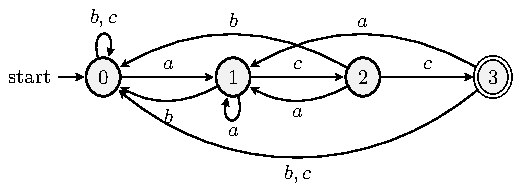
\includegraphics[width=0.35\textwidth]{./chapters/figures/forecasting/dfasr.pdf}
\label{fig:dfatcc}

\hfill

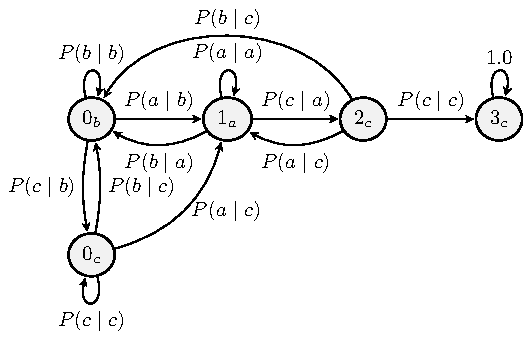
\includegraphics[width=0.35\textwidth]{./chapters/figures/forecasting/pmcr1.pdf}
\label{fig:mctcc1}

%\hfill
\caption{DFA and PMC for $\mathcal{P}=a ; c ; c$,  $\Sigma=\{a,b,c\}$, and order $m=1$  \cite{alevizos2017event}.}
\label{fig:dfa_mc_example}
\end{centering}
\end{figure}
%\end{comment}

\subsubsection*{Constructing Pattern Prediction Model}
\label{sec:pmc_prediction}

~\citet{alevizos2017event} proposed to use the constructed \pmcmr to build a probabilistic prediction model that describes the DFA's run-time behavior. The method is based on calculating the \textit{waiting-time} distributions. Given a specific state of the \pmcmr, a \textit{waiting-time} distribution provides the probability of reaching a set of absorbing states in $n$ transition from current state. So by mapping the final states of the DFA to absorbing states of the \pmcmr by adding self-loops with probabilities equal to $1.0$. Therefore, we can calculate the probability of reaching a final state in $n$ transitions,  which means predicting a full match of the defined pattern $\mathcal{P}$.

\par We denote by $W_{\mathcal{P}}(q)$  the waiting-time random variable that represents the
number of transitions until from a current state $q$ of DFA to reach a final state\cite{alevizos2017event}, which is given by 

\begin{equation*}
W_{\mathcal{P}}(q)=inf\{n: q_{0},q_{1},...,q_{n}, q_{0}=q, q \in Q \backslash F, q_{n} \in F\}
\end{equation*}

However, the \textit{waiting-time} distribution of the $W_{\mathcal{P}}(q)$ random variable can be computed based on the transition probability matrix $\Pi$ of the \pmcmr, where it has $h$ non-final states and $d$ final states (absorbing states) \cite{alevizos2017event}, then distribution is calculated by the following equation 

\begin{equation*}
P(W_{\mathcal{P}}(q)=n)=\boldsymbol{\xi_{q}}\boldsymbol{N}^{n-1}(\boldsymbol{I}-\boldsymbol{N})\boldsymbol{1}
\end{equation*}
where $\boldsymbol{N}$ is $h \times h$ matrix that obtained by re-arranging the transition matrix $\Pi$ to include transitions between the non-final states of the DFA, $\boldsymbol{I}$ is an identity matrix of size $d \times d$, and  $\boldsymbol{1}$ is $h \times 1$ vector of ones. The $\boldsymbol{\xi_{q}}$ is $1 \times h$ row of elements that contains zeros except $1.0$ in the cell corresponding to $q$. 
\par Finally, we provide the prediction reports in the form of intervals i.e.,  $I=(\mathit{start},\mathit{end})$. Which means that the DFA is expected to reach a final state in after future transitions between $\mathit{start}$ and $\mathit{end}$ with probability at least some constant threshold $\theta_{fc}$ that defined by the user. 
These intervals are estimated by a single-pass algorithm that scans a waiting-time distribution and finds the smallest (in terms of length) interval that exceeds this threshold. 
An example is shown in Figure \ref{fig:wtdfas},
where the DFA in Figure \ref{fig:dfa1} is in state $1$,
the \textit{waiting-time} distributions for all of its non-final states are shown in Figure \ref{fig:wt1}
and the distribution, along with the prediction interval, for state $1$ are depicted in green.
\begin{figure}[!ht]
\begin{centering}

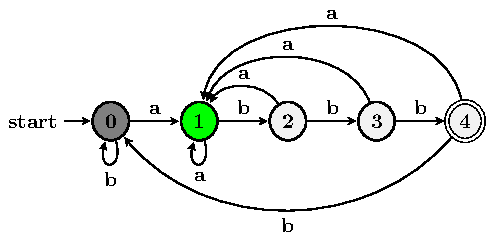
\includegraphics[width=0.19\textwidth]{./chapters/figures/forecasting/dfa1.pdf}
\label{fig:dfa1}


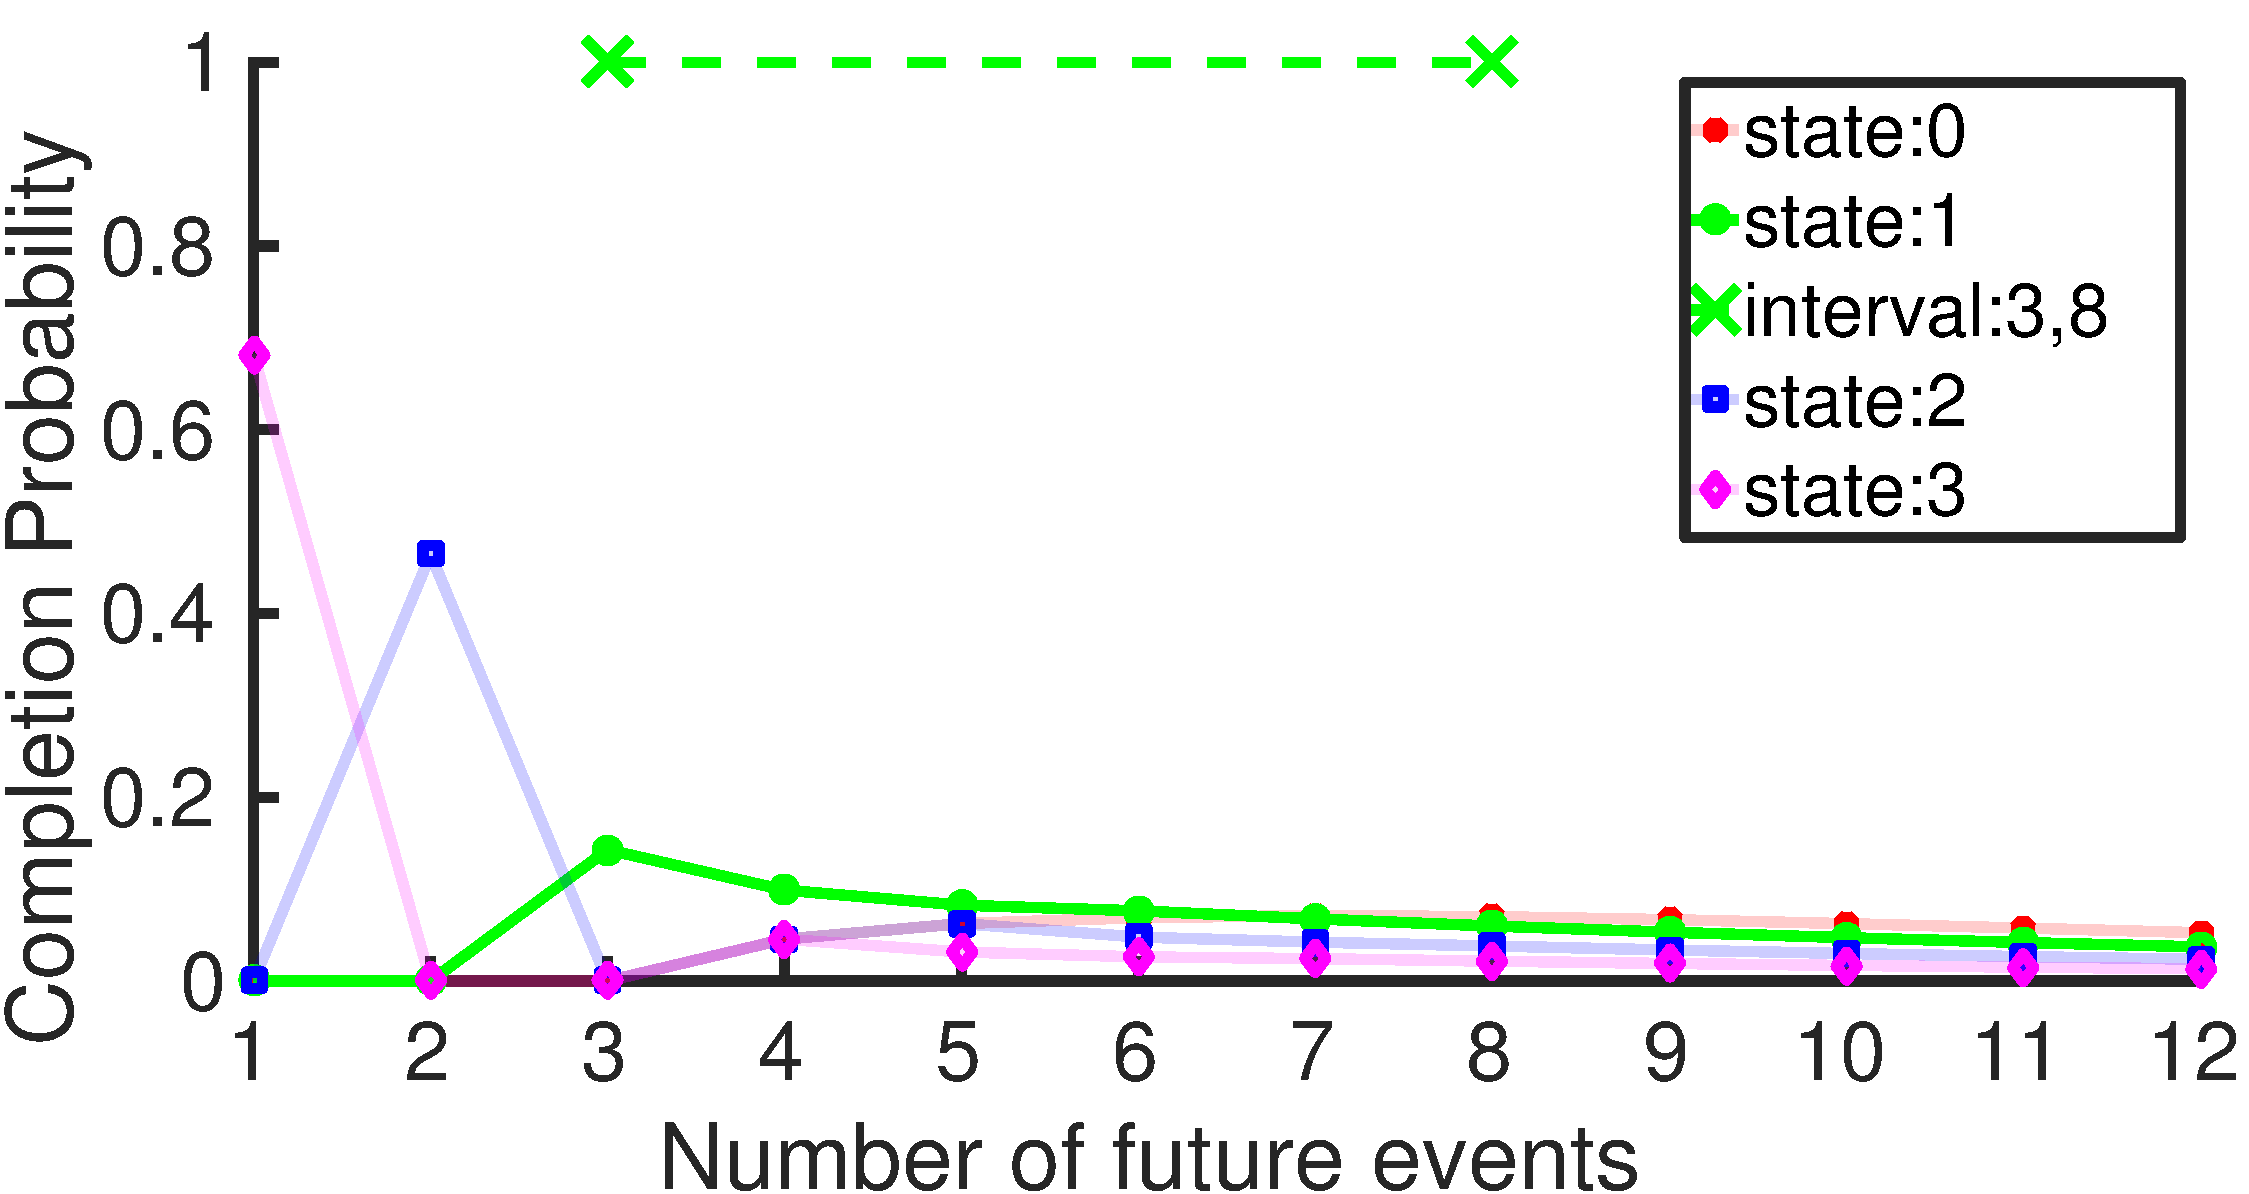
\includegraphics[width=0.28\textwidth]{./chapters/figures/forecasting/wt1.pdf}
\label{fig:wt1}

\caption{Example of how prediction intervals are produced. 
$\mathcal{P}=a ; b ; b ; b$, $\Sigma=\{a,b\}$, $m=1$, $\theta_{\mathit{fc}}=0.5$      \cite{alevizos2017event}.}
\label{fig:wtdfas}
\end{centering}
\end{figure}

\par The proposed method assumes that the transition probability matrix $\Pi$ is available to build the prediction intervals. However, this is not true in the real-world applications.
Therefore, it is essential to learn the values of the \pmcmr's transition probability matrix in order apply this method. One common way, is to use the maximum-likelihood estimator to learn the transition probabilities as illustrated in Section ~\ref{sec:theoretical}. This model is performing the learning over a single event stream $s$ that might requires a large amount of time until convergence to a sufficiently good model. In this thesis, we present a technique to distribute the learning of  transition probability matrix over multiple input event streams.

\section{Pattern Prediction on multiple Streams}

\subsection{Problem Formulation Extension}
Let $O = \{ o_1, ..., o_k\}$ be a set of \emph{$K$}  objects (i.e., moving objects) 
and $S = \{ s_1, ..., s_k\}$ a set of real-time streams of events,
where $s_i$ is generated by the object $o_i$.
Let $\mathcal{P}$ be a user-defined pattern which we want to apply to every stream $s_i$,
i.e., each object will have its own DFA.

\par The setting that is considered in this work is then described in the following:
we have \emph{$K$} input event streams $S$ and a system consisting of \emph{$K$} distributed predictor nodes $n_1,n_2...,n_k$, each of which consumes an input event stream $s_i\in S$. The goal is to provide timely predictions and be able to do this at large-scale.
Each node $n_i$ handles a single event stream $s_i$ associated with a moving object $o_i \in O$. In addition,  it  maintains a local prediction model $f_i$ for the user-defined pattern $\mathcal{P}$. The $f_i$ model provides the online prediction about the future full match of the pattern $\mathcal{P}$ in $s_i$  for each new arriving event tuple. 
\par In short, we have multiple running instances of an online prediction algorithm on distributed nodes for multiple input event streams. More specifically, the input to our system consists of massive streams of events  that describe trajectories of moving vessels in the context of maritime surveillance, where there is one predictor node for each vessel's event stream.
  
%
%The defined pattern $\mathcal{P}$ is monitored over each event stream $s_i$  by a  predictor nodes  $n_i$  that maintains a local prediction model $f_i$, where there is one node for each vessel's event stream.  The prediction model $f_i$ gives the ability to provide an online predictions about when the pattern will be completed in the form of an expected number of future events before a full match does occur.

\subsection{Proposed Approach}
\label{sec:proposed_approach}
\par We design and develop a scalable and distributed patterns prediction system over a massive input event streams of moving objects. As the base prediction model, we use the PMC forecasting method \cite{alevizos2017event}. Moreover, we propose to enable the information exchange between the distributed predictors/learners of the input event streams, by adapting the distributed online prediction protocol of \cite{kamp2014communication} to synchronize the prediction models, i.e., the transitions probabilities matrix of the PMC predictors.

\par Algorithm~\ref{algonline:dol} presents the distributed online prediction protocol by dynamic model synchronization on both the predictor nodes and the coordinator. We refer to the PMC's transition matrix $\boldsymbol{\Pi}_i$ on predictor node $n_i$ by $f_i$. That is, when a predictor $n_i:\ i \in[k]$ observes an event $e_j$ it revises its internal model state (i.e., $f_i$) and provides a prediction report. Then it checks the local conditions  (batch size $b$ and local model divergence from a reference model $f_r$) to decide whether there is a need to synchronize its local model with the coordinator [or not].  $f_r$ is maintained in the predictor node as a copy of the last computed aggregated model $\hat{f}$ from the previous full synchronization step, which is shared between all local predictors/learners. By monitoring the local condition $\|f_i - f_r\|^2 > \Delta$ on all local predictors, we have a guarantee that if none of the local conditions is violated, the divergence (i.e., variance of local models $\delta(f)=\frac{1}{k} \sum_{j=1}^{k}\|f_i - \hat{f}\|^2$) does not exceed the threshold $\Delta$ \cite{kamp2014communication}. 

\par On the other hand, the coordinator receives the prediction models from the predictor nodes that requested for model synchronization (violation). Then it tries to keep incrementally querying other nodes for their local prediction models until reaching out all nodes, or the variance of the aggregated model $\hat{f}$ that is computed from the already received models less or equal than the divergence threshold  $\Delta$. Finally, the aggregated model $\hat{f}$ is sent back to the predictor nodes that sent their models after the violation or have been queried by the coordinator.

\begin{algorithm}[h]
	\caption{Communication-efficient Distributed Online Learning \cite{kamp2014communication}.} 
	\begin{algorithmic}[1] 
		\Statex \Indm  \textbf{Predictor} node $n_i$: at observing event $e_j$
		\Statex \Indp update the prediction model parameters $f_i$ and provide a prediction service \; 

		\Statex \If {$j\mod b = 0\ and\ \|f_i - f_r\|^2 > \Delta$}  
		\Statex send  $f_i$ to the Coordinator (violation) \;
		\Statex \Indm \textbf{Coordinator}:
		\Statex \Indp receive local models with violation 
		 $B=\{f_i\}_{i=1}^m$ \;
	
	
		\Statex \While{$|B| \neq k $ and $\frac{1}{|B|} \ \sum_{f_i\in  \Pi}\|f_i - \hat{f}\|^2 > \Delta$}{
			
			 \Statex  \hspace{\algorithmicindent} add other nodes have not reported violation for \Statex \hspace{\algorithmicindent} their models $ B \gets \{f_l : f_l \notin B\ and\ l \in [k]\}$    \;
			\Statex  \hspace{\algorithmicindent} receive models from nodes add to $B$\;
	}
        \Statex
		\Statex compute a new global model $\hat{f}$ \;
		\Statex send $\hat{f}$ to all the predictors in $B$ and set $f_{1}\dots f_{m}=\hat{f} $\; 
		\Statex \If {$|B| = k$}{
		\Statex  \hspace{\algorithmicindent} set a new reference model $f_r	\gets \hat{f}$ \; }
	
	\end{algorithmic}
	\label{algonline:dol}
\end{algorithm}


\par  We use this protocol for the pattern prediction model, which is internally based on the PMC \pmcmr. This allows the distributed \pmcmr\ predictors for multiple event streams to  synchronize their models (i.e., the transition probability matrix of each predictor) within the system in a communication-efficient manner. 



\par We propose a \textit{synchronization operation} for the parameters of the models ($f_i=\boldsymbol{\Pi}_i :i \in[k]$) of the $k$ distributed PMC predictors. The operation is based on distributing the maximum-likelihood estimation \cite{anderson1957statistical} for the transition probabilities of the underlying \pmcmr\ models described by: 
\begin{equation}
\label{eq:dis_pi_estim}
\hat{\pi}_{i,j}=\frac{\sum_{k \in K} n_{k,i,j}}{\sum_{k \in K} \sum_{l \in L} n_{k,i,l}}
\end{equation}

\par Moreover, we measure the divergence of local models from the reference model  $\|f_k - f_r\|^2$ by calculating the sum of square difference between the transition probabilities  $\boldsymbol{\Pi}_i$ and  $\boldsymbol{\Pi}_r$:
\begin{equation*}
\label{eq:dis_pi_varinace}
\|f_k - f_r\|^2=\sum_{i,j} (\hat{\pi}_k{i,j} -\hat{\pi}_r{i,j})^2
\end{equation*}
\par In general, our approach relies on enabling the collaborative learning between the prediction models of  the input event streams. By doing so, we assume that the underlying event streams belong to the same  distribution and share the same behavior (e.g., mobility patterns). We claim this assumption is reasonable in many application domains: for instance, in the context of maritime surveillance, vessels travel through standard routes, defined by the International Maritime Organization (IMO). Additionally, vessels have similar mobility patterns in specific areas such as moving with low speed and multiple turns near the ports \cite{pallotta2013vessel,liu2014knowledge}. That allows our system to construct a coherent global prediction model dynamically for all input event streams based on merging their local prediction models.

% may add it to conclusion 
%\par By enabling collaborative learning our approach is imposing an acceleration of learning of the underlying prediction models with less training data, in addition, it provides an improvement of the predictive performance compared to the no-distributed  version of event forecasting with Pattern Markov Chains system. 

\section{Analysis of the Proposed Approach}

\subsection{General  Overview}
\par Generally, our approach relies on enabling the collaborative learning among the distributed predictors. Each predictor node receives a stream of events related to a distinct moving object, and the central coordinator is responsible of synchronizing their prediction models using the \textit{synchronization operation}. Moreover, the predictors they only need to share the parameters of their models without aggregating all input event streams. 

\par In addition, our approach relies on enabling the collaborative learning between the prediction models of the input event streams. By doing so, we assume that the underlying event streams belong to the same  distribution and share the same behavior (e.g., mobility patterns). We claim this assumption is reasonable in many application domains: for example, in the context of maritime surveillance, vessels travel through standard routes, defined by the International Maritime Organization (IMO). Additionally, vessels have similar mobility patterns in specific areas such as moving with low speed and multiple turns near the ports \cite{pallotta2013vessel,liu2014knowledge}. That allows our system to construct a coherent global prediction model dynamically for all input event streams based on merging their local prediction models.

\par The underlaying learning process is based on estimating the transition probability matrix of the \pmcmr models, where the maximum-likelihood estimator  \cite{anderson1957statistical} is used to learn the transition probability matrix for each \pmcmr. In our approach, we propose a synchronization operation (Equation ~\ref{eq:dis_pi_estim}) to build a global estimation of the transition probability matrix among the \emph{$K$} predictors. In next, we present the maximum-likelihood estimator, and we  provide a theoretical analysis of the proposed operation, where we further present a probabilistic guarantee of the efficiency of our distributed learning estimation against the isolated estimations.   
% may add it to conclusion 
%\par By enabling collaborative learning our approach is imposing an acceleration of learning of the underlying prediction models with less training data, in addition, it provides an improvement of the predictive performance compared to the no-distributed  version of event forecasting with Pattern Markov Chains system. 


\subsection{Theoretical Analysis}
\label{sec:theoretical}

 In this section, we present preliminaries of the Markov chain models and the maximum-likelihood estimator of the transition probabilities, and we describe the theoretical properties of our proposed synchronization operator and its relation with the maximum-likelihood estimator. Also, we derive a probabilistic guarantee of our method estimations for the transition probabilities. 
 
 
 \subsubsection*{Preliminaries}
 We first give a brief introduction to the Markov chain theory, where the theoretical definitions and notations presented are based on the work described in \cite{bertsekas2002introduction,Billingsley1961,anderson1957statistical,howard2012dynamic}.

\begin{definition}
	Let $\{q_0, q_1, \ldots q_n\}$ be a sequence of random variables as \textbf{Markov chain}, where the variable $q_i$ belongs to a finite state space $\mathbf{S =\{1,\ldots m\}}$ and represents the observed state of the chain at time $i$. Let the transition probabilities of the Markov chain $p_{ij}(t+1)$ such that $i,j \in S$ and $t=0,\ldots, n$, where  $p_{ij}(t+1)$ is the probability of the state $j$ at time $t+1$, given  state $i$ at time $t$, then the sequence $\{q_0, q_1, \ldots q_n\}$ satisfies the \textbf{Markov property} 
	
	\begin{equation}
	\begin{aligned}
	P(q_{t+1}=j|q_{t}=i,q_{t-1}=i_{t-1},\ldots ,q_{0}=i_{0})=P(q_{t+1}=j|q_{t}=i)\\
	\forall i,j,i_{t-1},i_{0} \in S
	\end{aligned}
	\end{equation}

\end{definition}



\par That is, the probability of moving to a future state only depends on the current state (Markov chain of order $1$). While for higher order $m$ Markov chains the conditional probabilities are modeled to be dependent on the last $m$ states. 

\par When the conditional probabilities $P(q_{t+1}=j|q_{t}=i)$ are independent of the time $t$, the Markov chain is called \textbf{homogeneous} such that $p_{ij}:=P(q_{t+1}=j|q_{t}=i)$.

The transition probabilities of the Markov chain are represented by a $m \times m$ matrix that called \textbf{transition probability matrix} $\boldsymbol{\Pi}$ with $p_{ij}$ elements


\begin{equation}
\label{eq:matrix_example}
\boldsymbol{\Pi} = 
\begin{bmatrix} 
p_{1,1}	   &p_{1,2}  &. 		&. 		& . &  	p_{1,m} \\
p_{2,1}		   &.  & .		& .	    & .	& . \\
. 		   &.  & .		& .	    & .	& . \\
.		   &.  & .		& .		& .	& . \\
.		   &.  & .		& .		& .	& .\\
p_{m,1}	   & p_{m,1}	&.		& .	& .	&p_{m,m}
\end{bmatrix}
\end{equation}

where $0 \leq p_{i,j}\leq 1 $ and the rows sum up to one 
\begin{equation}
\sum_{j=1}^{m} p_{i,j}= 1\ \ \ \ \ \ \ \ \ i=1,2 \ldots m
\end{equation}

\subsection{Learning the Transition Probability Matrix for a Single Markov Chain}
 \
\par As mentioned in Section ~\ref{sec:pmc_prediction}, we rely on the transition probability matrix of \pmcmr to build the prediction intervals. Given that the sequence of the states $\{q_0, q_1, \ldots q_n\}$ that DFA visits after consuming the input event stream is a 1-order Markov chain.


\par However, in practice the underlying transition probability matrix is unknown, and desirable to estimate or learn it form the observed sequence $\{q_0, q_1, \ldots q_n\}$. The maximum-likelihood estimator is a common method to estimate the transition probability matrix \cite{anderson1957statistical}.


\begin{definition}
	Let $\boldsymbol{\Pi}$ is the transition probability matrix of a single Markov chain with a set of states $S$, 
	$\pi_{i,j}$ the transition probability from state $i$ to state $j$,
	$n_{i,j}$ the number of observed transitions from state $i$ to state $j$,
	then the maximum-likelihood finds $\boldsymbol{\hat{\Pi}}$ as an estimate for $\boldsymbol{\Pi}$, where its elements $\hat{p}_{i,j}$ are
	\begin{equation}
	\label{eq:pi_estim}
	\hat{p}_{i,j}=\frac{n_{i,j}}{\sum_{l \in S} n_{i,l}}=\frac{n_{i,j}}{n_{i}}
	\end{equation}
	
\end{definition} 

Where this estimator is used separately to learn each transition probability matrix of all \pmcmr models.   


\textbf{Proprieties of the maximum-likelihood estimates}. 
	The maximum likelihood estimates of transition probabilities of a single sequence $\{q_0, q_1, \ldots q_n\}$  are obtained based on the observed transitions between the states of the chain. That is, the maximum likelihood estimates are basically the count of transitions from $i$ to $j$ divided by the total count of the chain being in state $i$.  
	
	\par ~\citet{anderson1957statistical} have shown that 
	
	
%	\begin{equation}
%	\label{eq:lim_dist}
%	\lim_{n\to\infty} \sqrt{n}\ (\hat{p}_{i,j} - {p}_{i,j}) \sim \mathcal{N}(\mu,\,\sigma^{2}_{mle})\,.
%	\end{equation}

	\begin{equation}
	\begin{aligned}
	\label{eq:lim_dist}
	 \sqrt{n}\ (\hat{p}_{i,j} - {p}_{i,j}) \xrightarrow{d} \mathcal{N}(\mu,\,\sigma^{2})\\
	 as\ n \xrightarrow{} \infty
	 \end{aligned}
	\end{equation}
Thus, the random variable $\sqrt{n}\ (\hat{p}_{i,j} - {p}_{i,j})$ has asymptotically normal distribution with mean $\mu=0$, and  variance  $\sigma^{2}$ is given by   

\begin{equation}
\begin{aligned}
\sigma^{2}=\mathrm{Var}(\sqrt{n}\ (\hat{p}_{i,j} - {p}_{i,j})) = \frac {{p}_{i,j}\ (1- {p}_{i,j})} {\phi_{i}} \\
\text{s.t.}\ \phi_{i} = \sum_{l=1}^{m} \sum_{t=1}^{n} \eta_{l} \ p_{l,j}^{t-1}
\end{aligned}
\end{equation}

Where $p_{l,j}^{t-1}$ is the probability of state $j$ at time $t-1$ given that the state $l$ at time $0$ ~\cite{anderson1957statistical}. We are interested in the variances of $(\hat{p}_{i,j} - {p}_{i,j})$ that represents the error in the estimation of ${p}_{i,j}$ by the maximum-likelihood estimator, which is given by:

	\begin{equation}
\begin{aligned}
\label{eq:var_isol}
	\mathrm{Var} (\hat{p}_{i,j} - {p}_{i,j}) =  \frac {\mathrm{Var}(\sqrt{n}\ (\hat{p}_{i,j} - {p}_{i,j}))}{n} = \frac {\sigma^{2}}{n} 
\end{aligned}
\end{equation}

It is clearly seen that variances are dropping as the sample size $n$ grows large.  In next, we will show that our proposed approach of synchronizing the maximum likelihood estimators over $k$ chains is preserving  a similar asymptotic behavior and gives efficient estimates of the transition probabilities.


\subsubsection{Probabilistic Learning Guarantee}
 %in Equation ~\ref{eq:dis_pi_estim}% 
\par The proposed synchronization operator is aggregating the maximum-likelihood estimates over $k$ observed sequences (i.e., sequences of the DFA states based on the consumed event streams), the operator estimates a global transition probabilities matrix for a set of $k$ sequences, which are arranged in serial order as one large chain with length $N=k*n$, where we assume that all $k$ sequences have $n$ observations. For the sake of simplicity, we assume that the synchronization phase happens on batch size equals $n$ (i.e., $b=n$) given that the $\Delta$ is zero, then the global transition probabilities $\hat{\pi}_{i,j}$ are given 
\begin{equation}
\label{eq:dis_pi_estim2}
	\begin{aligned}
\hat{\pi}_{i,j}=\frac{\sum_{k \in K} n_{k,i,j}}{\sum_{k \in K} \sum_{l \in L} n_{k,i,l}} = \hat{p}_{i,j}(N)\\\\
 where\ N = k*n.
 \end{aligned}
\end{equation}
%This is equivalent to

\par Thus, this operation it allows to observe more samples, which is naturally producing a better estimates of the transition probabilities. In addition, our proposed synchronization operation of the $k$ transition matrices has the same proprieties as the maximum likelihood estimator over a serial sequence of all $k$ sequences, but with skipping $k-1$ transitions between each two consecutive sequences, which is in practice a small number that can be neglected comparing to the total transitions count $k*n$. As result, the global transition probabilities of our approach  have the same properties as maximum likelihood estimates, in particular, the the random variable $\sqrt{N}\ (\hat{\pi}_{i,j} - {p}_{i,j})$ has asymptotically normal distribution with mean $\mu=0$, and  following Equation ~\ref{eq:lim_dist} we have variance 

\begin{equation}
\begin{aligned}
\label{eq:lim_dist2}
\sqrt{N}\ (\hat{\pi}_{i,j} - {p}_{i,j}) \xrightarrow{d} \mathcal{N}(0,\,\sigma^{2})\\
as\ N \xrightarrow{} \infty\\
where\ N = n*k .\\
\end{aligned}
\end{equation}

So, 
\begin{equation}
\begin{aligned}
\label{eq:var_sync}
 \mathrm{Var} (\hat{\pi}_{i,j} - {p}_{i,j}) = \frac {\sigma^{2}}{N} =  \frac {\sigma^{2}}{k*n}
\end{aligned}
\end{equation}


That is, since $N > n$ combining $k$ sequences, the variances of estimations of our method  $\mathrm{Var} (\hat{\pi}_{i,j} - {p}_{i,j})$ are smaller than the estimates of maximum-likelihood over a single sequence $\mathrm{Var} (\hat{p}_{i,j} - {p}_{i,j})$. 
\par Thus, it follows from the  Chebyshev's inequality \cite{feller1968introduction} that we have for the random variable $\hat{p}_{i,j} - {p}_{i,j}$, for any constant $c > 0$  

\[ \Pr\left( |(\hat{p}_{i,j} - {p}_{i,j}) - \mu| \geq c \right) \leq
\frac{\mathrm{Var} (\hat{p}_{i,j} - {p}_{i,j})}{c^2} \]


 The mean $\mu=0$ is zero and the $\mathrm{Var} (\hat{p}_{i,j} - {p}_{i,j})$ equals  $\frac {\sigma^{2}}{n}$, and therefore 
 
 \[ \Pr\left( |\hat{p}_{i,j} - {p}_{i,j}| \geq c \right) \leq
 \frac{\sigma^{2}}{c^2 * n} \]
 
 
$\hat{p}_{i,j} - {p}_{i,j}$  represents the deviation/error between the estimates of maximum-likelihood over a single (i.e., isolated) sequence and the true probabilities. On the other hand, we can obtain, in the same way, the probability bound of deviations for our synchronization operator estimates as follows:

\[ \Pr\left( |\hat{\pi}_{i,j} - {p}_{i,j}| \geq c \right) \leq
\frac{\sigma^{2}}{c^2* n*k} \]


\par Using Equation~\ref{eq:var_sync} we obtain the value $\mathrm{Var} (\hat{\pi}_{i,j} - {p}_{i,j})$, and Equation~\ref{eq:var_sync} for $\mathrm{Var} (\hat{p}_{i,j} - {p}_{i,j})$. Given that $k \ge 1$, then  the variance of $\hat{\pi}_{i,j} - {p}_{i,j}$  is less than or equal to the variance of $\hat{p}_{i,j} - {p}_{i,j}$

\[ 
\frac{\sigma^{2}}{c^2 *n*k} \leq
\frac{\sigma^{2}}{c^2 * n}
 \]

So, we have for any constant $c > 0$ and $k \ge 1$, a probabilistic learning guarantee of the transition probabilities: 

\[ \Pr\left( |\hat{\pi}_{i,j} - {p}_{i,j}| \geq c \right) \leq
 \Pr\left( |\hat{p}_{i,j} - {p}_{i,j}| \geq c \right)
 \]
 where $\hat{p}_{i,j}$ a transition probability, which is learned on a single \pmcmr predictor, and the $\hat{\pi}_{i,j}$ is the global transition probability that computed by the synchronization operation (Equation ~\ref{eq:dis_pi_estim}). To summarize, our approach is based aggregating the maximum-likelihood estimates over $k$ sequences, which speeds up the convergence to reach the true transition probabilities as result of the smaller variances of the estimates.

%The weak law of large
%numbers states that, if $X_1, X_2, X_3, \ldots$ are independent and identically
%distributed random variables with mean $\mu$ and standard deviation $\sigma$,
%then for any constant $\epsilon > 0$ we have 
%%
%\[ \lim_{n \rightarrow \infty} \Pr \left( \left| \frac{X_1 + X_2 + \cdots +
%	X_n}{n} - \mu \right| > \epsilon \right) = 0. \]
%Use Chebychev's inequality to prove the weak law of large numbers.

 
\subsection{Transition Matrix of the Underlaying Markov Chain}
\label{sec:underlaying_mc}
\par In order to empirically study the learning efficiency of our distributed learning based proposed approach against the isolated approach, we need to map the transition probabilities of the underlying Markov chain with the transition probability matrix ($\hat{\Pi}$) of the \pmcmr model. ~\citet{nuel_pattern_2008} showed in \textbf{Theorem 3} the relation between the elements  of 
$\Pi$ and the conditional probabilities of the $m-$order Markov chain $X=\{X_1, X_2, \ldots X_n\}$ described by 

\[ \Pi(p, q) =
\begin{cases}
P(X_{m+1}=b|X_1\ldots X_m=\delta^{-m}(p))     & \quad \text{if } \delta(p,q)=b \\
0  & \quad \text{if } p \notin  \delta(p,X)
\end{cases}
\]
Using this theorem, in the case of the underlaying transition probability matrix is known (e.g., synthetic event streams),  we then can compare the estimation efficiency of the different approaches for the transition probabilities of the underlaying Markov chain $X$.  For example, the transition probability matrix of the \pmcmr model for the pattern $\mathcal{P}=a ; d ; c$ over  $\Sigma=\{a,b,c,d\}$ is represented by: 

\begin{equation}
\label{eq:matrix}
\boldsymbol{\Pi} = 
\begin{Bmatrix} 
 1          \\ 2        \\3             \\4         \\5         \\ 6 
\end{Bmatrix}
\begin{bmatrix} 
P(a|a) 	& P(b|a) 		& P(c|a) 		& 0			  & p(d|a) 	& 0  \\
P(a|b) 	& P(b|b) 		& P(c|b) 		& P(d|b)	  & 0 	    & 0  \\
P(a|c) 	& P(b|c) 		& P(c|c) 		& P(d|c) 	  & 0 	    & 0  \\
P(a|d) 	& P(b|d) 		& P(c|d) 		& P(d|d)	  & 0 	    & 0  \\
P(a|d) 	& P(b|d) 		&  0	 	    & P(d|d)	  & 0 	    & P(c|d)  \\
0			& 0			& 0		        & 0    		  & 0		& 1.0
\end{bmatrix}
\end{equation} 

%ADD figure example for the figure in the PMC section%
	
	

\chapter{System Overview}
\label{chapter:overview}
%ADD more details and interfacse structure%
%CHECK Towards Flexible Event Processing in Distributed Data Streams%
%SEE delevriable%
\section{System Architecture}
\label{sec:architecture}
Our system consumes as an input\footnote{In practice, the aggregated input events stream is composed of multiple event streams (partitions) from a set of moving objects.} an aggregated stream of events coming from a large number of moving objects, which is continuously collected and fed into the system. It allows users to register a pattern $\mathcal{P}$ to be monitored over each event stream of a moving object. The output stream consists of original input events and predictions of full matches of $\mathcal{P}$, displayed to the end users. Figure ~\ref{fig:architecture} presents the overview of our system architecture and its main components.      


\begin{figure}[h]
	
	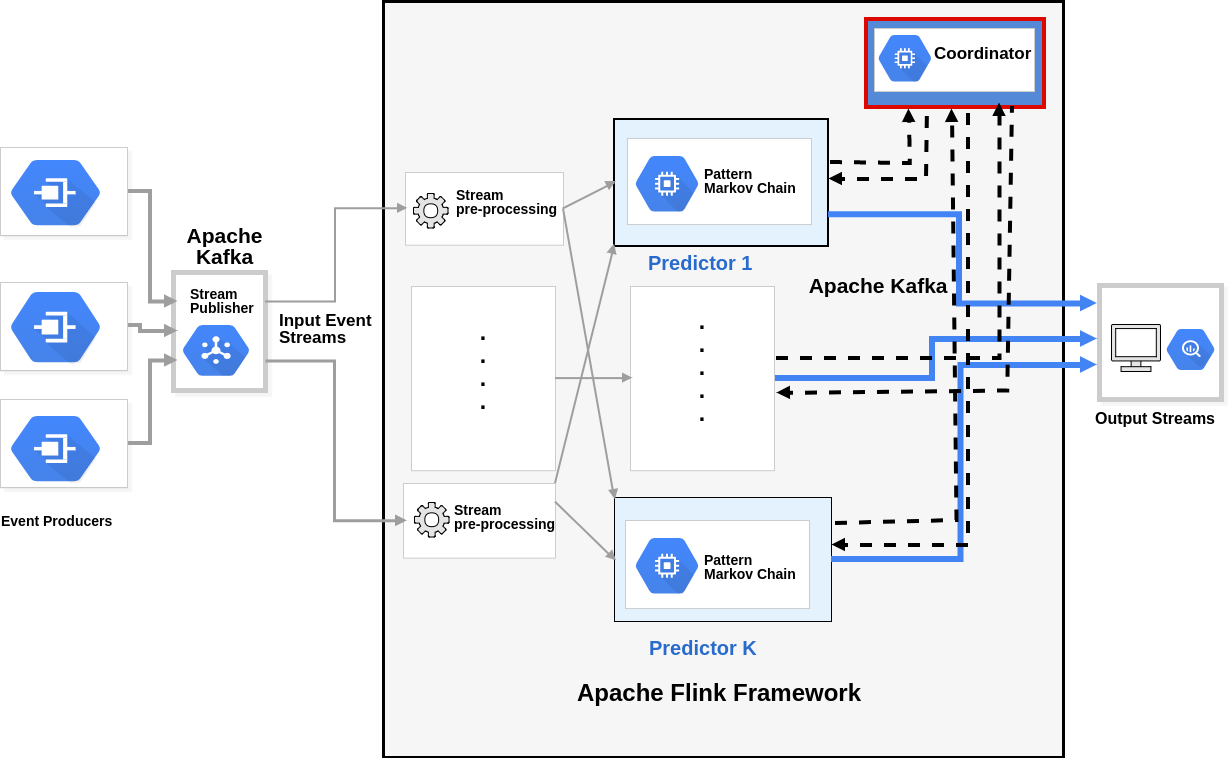
\includegraphics[width=\linewidth]{chapters/figures/system.png}
	
	\caption{System architecture overview.}
	\label{fig:architecture}
\end{figure}

The system is composed of three processing units:   \begin{enumerate}[]
	\item pre-processing operators that receive the input event stream and perform filtering and ordering operations, before partitioning the input event stream to multiple event streams based on the associated moving object 
	\item predictor nodes (learners), which are responsible for maintaining a prediction model for the input event streams. Each prediction node is configured to handle an event stream from the same moving object, in order to provide online predictions for a predefined pattern $\mathcal{P}$  
	\item a coordinator node that communicates through Kafka stream channels with the predictors to realize the distributed online learning protocol. It builds a global prediction model, based on the received local models, and then shares it among the predictors.
\end{enumerate}

\par Our distributed system consists of multiple pre-processing operators, prediction nodes, and a central coordinator node. All units run concurrently and are arranged as a  data processing pipeline, depicted in Figure ~\ref{fig:architecture}. We leverage Apache Kafka as a messaging platform to ingest the input event streams and to publish the resulting streams. Also, it is used as the communication channel between the predictor nodes and the coordinator. Apache Flink is employed to execute the system's distributed processing units over the input event streams: the pre-processing operators,  the prediction units, and the coordinator node. Our system architecture can be modeled as a logical network of processing nodes, organized in the form of a DAG, inspired by the Flink runtime dataflow programs \cite{carbone2015apache}. 

\section{Implementation Details}
\label{sec:impl}
In this section, we describe in detail the implementation of our system. It has been implemented on top of Apache Flink and Apache Kafka frameworks. Each of the three sub-modules, described in Section ~\ref{sec:architecture}, have been implemented as Flink operations over the input events stream. 

\textbf{Pre-processing and Prediction Operators.} Listing ~\ref{algonline:flink1} shows how the main workflow of the system is implemented as Flink data flow program.

The system ingests the input events stream from a Kafka cluster that is mapped to a \textit{DataStream} of events, which is then processed by an \textit{EventTuplesMapper} to create tuples of \textit{(id, event)}, where the \textit{id} is associated to the identifier of the moving object. To handle events  coming in out of order in a certain margin, the stream of event tuples  is processed by a \textit{TimestampAssigner}, it assigns the timestamps for the input events based on the extracted creation time. Afterwards,  an ordered stream of event tuples is generated using a process function \textit{EventSorter}.

	\begin{lstlisting}[caption={Flink pipeline for local predictors workflow},label={algonline:flink1},frame=single]
	DataStream<Event> eventsStream = env.addSource(kafkaConsumer);	
	// Create event tuples (id,event) and assign time stamp 
	DataStream<Tuple2<String,Event>> eventTuplesStream =
	inputEventsStream.map(new EventTuplesMapper())
	.assignTimestampsAndWatermarks(new EventTimeAssigner());	
	// Create the ordered keyed stream 
	 keyedEventsStream = eventsStream.keyBy(0).process(new EventSorter()).keyBy(0);	
	//Initialize the predictor node 
	LocalPredictorNode predictorNode =new LocalPredictorNode<Event>(P);
	// Process the  keyedEventsStream by the predictor 
	DataStream<Event> processedEventsStream =
	keyedEventsStream.map(predictorNode);
	\end{lstlisting}
	
\par The ordered stream is then transformed to a \textit{keyedEventsStream} by partitioning it, based on the ids values, using a \textit{keyBy} operation. A local \textit{predictor} node in a distributed environment is represented by a \textit{map} function over the \textit{keyedEventsStream}. Each parallel instance of the map operator (predictor) always processes all events of the same moving object (i.e., equivalent id), and maintains a bounded prediction model (i.e., \pmcmr\  predictor) using the Flink's Keyed State  \footnote{{Keyed State in Flink: \url https://ci.apache.org/projects/flink/flink-docs-release-1.3/dev/stream/state.html\#kayed-state}}.  The output streams of the moving objects from the parallel instances of the predictor map functions are sent to a new Kafka stream (i.e., same topic name).  They then can be processed by other components like visualization or users notifier.


\par Moreover, the implementation of  the \textit{predictor} map function includes the communication  with \textit{coordinator} using Kafka streams. At the beginning of the execution, it sends a registration request to the coordinator. Also at the run-time,  it sends  its local prediction model as synchronization request,  or as a response for a resolution request from the coordinator. These communication messages are published into different Kafka topics as depicted in Table ~\ref{tab:messagesToTopics}. 
\begin{center}
\centering
\begin{table}[h]
	\caption{Messages to Kafka topics mapping.}
	\label{tab:messagesToTopics}
	\begin{tabular}{p{5cm}l}
		\toprule
		Message &Kafka Topic\\
		\midrule
		\parbox[t]{4cm}{\textit{RegisterNode}, \\ \textit{RequestSync}, and \\\textit{ResolutionAnswer} } &LocalToCoordinatorTopicId\\ \\
		
			  \parbox[t]{4cm}{\textit{CoordinatorSync} and \\ \textit{RequestResolution}} &CoordinatorToLocalTopicId\\
		\bottomrule
	\end{tabular}
\end{table}

\end{center}

\textbf{Coordinator.} Listing ~\ref{algonline:flink2} presents the workflow of the coordinator node that manages the distributed online learning protocol operations, which is implemented as Flink program. The coordinator receives messages from the local predictors through a Kafka Stream of a topic named \textit{"LocalToCoordinatorTopicId"}. It is implemented as a single \textit{map} function over the messages stream, by setting the \textit{parallelism} level of the Flink program to \textit{"1"}. Increasing the parallelism will scale up the number of parallel coordinator instances, for example, in order to handle different groupings of the input event streams. The map operator of the coordinator  handles three message types from the predictors: \begin{enumerate}[]
	\item \textbf{RegisterNode} that contains  a registration request for a new predictor node,
	\item \textbf{RequestSync} to receive a local model after violation,
	\item \textbf{ResolutionAnswer} to receive a resolution response from a local predictor node.  
\end{enumerate}  
 In addition, it sends \textbf{CoordinatorSync} messages for all predictors after creating a new global prediction model, or \textbf{RequestResolution} to a ask the local predictors for their prediction models.
 

\begin{lstlisting}[caption={The coordinator Flink program.},label={algonline:flink2},frame=single]
    streamExecutionEnvironment.setParallelism(1);
	// Read messages from local predictors
	DataStream<TopicMessage> messagesStream = readKafkaStream(env, "LocalToCoordinatorTopicId");	
	// Initialize the coordinator node
	CompunctionEfficientCoordinator coordinatorNode = new CompunctionEfficientCoordinator(configs);
	// Ingest the messages stream by the coordinator	
	DataStream<CoordinatorMessage> coordinatorMessagesStream = messageStream.map(coordinatorNode);	
	// Send the messages from the coordinator to the local predictors
	writeKafkaStream(coordinatorMessagesStream, CoordinatorToLocalTopicId);
\end{lstlisting}
       

	\chapter{Empirical Evaluation}

\label{chapter:evaluation}

\section{Evaluation Over Synthetic Event Streams}

\section{Evaluation Over Real-word Event Streams}
\label{sec:results}
In this section, we evaluate our proposed system by analyzing the predictive performance and communication complexity  using real-world event streams provided by the datAcron project in the context of maritime monitoring. The used event streams describe critical points (i.e., synopses) of moving vessels trajectories, which are derived from raw AIS messages as described in \cite{synopses1}. In particular, for our evaluation experiments we used a data set of synopses that contains $4,684,444$ critical points of $5055$ vessels sailing in the Atlantic Ocean during the period from 1 October 2015 to 31 March 2016.

\par We used the synopses data set to generate a simulated stream of event tuples  i.e., \textit{(id, timestamp, longitude, latitude, annotation, speed, heading)}, which are processed by the system to attach an extra attribute \textit{type} that represents the event value,  where $type$ $\in \Sigma$,  and $ \Sigma= \Sigma_1=$$\{$\textit{VerySlow, Slow, Moving,  Sailing, Stopping}$\}$ , which is based on a discretization of the speed values. Or $\Sigma=\Sigma_2=$ $\{$\textit{stopStart, stopEnd, changeInSpeedStart, changeInSpeedEnd,  slowMotionStart, slowMotionEnd, gapStart, gapEnd, changeInHeading}$\}$, which is derived based on the values of the $annotation$ attribute that encodes the extracted trajectory movement events \cite{synopses1}. In our experiments, we monitor a pattern $\mathcal{P}_1=Sailing$ with $\Sigma_1$ that detects when the vessel is underway (sailing). Likewise, we test a second pattern  $\mathcal{P}_2=$\textit{changeInHeading; gapStart; gapEnd; changeInHeading} with $\Sigma_2$.


\subsection*{Experimental setup} We ran our experiments on single-node standalone Flink cluster deployed on an Ubuntu Server 17.04 with Intel(R) Core(TM) i7-7700 CPU @ 3.60GHz X 8 processors and 32GB RAM. We used Apache Flink v1.3.2 and Apache Kafka v0.10.2.1 for our tests.


\subsection*{Evaluation criteria} Our goal is to evaluate our distributed pattern prediction system, which enables the synchronization of prediction models (i.e., PMC models) on the distributed predictor nodes. Our proposed system can operate in three different modes of  protocols/schemes of models synchronization: \begin{enumerate}[]
	\item static scheme based on synchronizing the prediction models periodically every $b$ of input events in each stream, 
\item continuous, full synchronization for each incoming event (hypothetical), 
\item dynamic synchronization protocol based on making the predictors communicate their local prediction models periodically but only under condition that the divergence of the local models from a reference model exceeds a variance threshold $\Delta$ (recommended).  	   

\end{enumerate}
\par We compare our proposed system against the isolated prediction mode, in which models are computed on single streams only, and compare the predictive performance in terms of :
\begin{enumerate}[]
	
\item  $\mathit{precision} =$ $ \mathit{\frac{\#\ of\ correct\ predictions}{\#\ of\ total\ predictions}}$ is the fraction of the produced predictions that are correct (i.e., a full match occurred within the prediction interval).   

\item $\mathit{spread} =end(I) -start(I)$ is the width of the prediction interval $I$. 

\end{enumerate} 
\par Moreover, we study the communication cost by measuring the $\mathit{cumulative\ communication}$ that captures the number of messages, which are required to perform the distributed online learning modes to synchronize the prediction models. Next, we present the experimental results for the patterns  $\mathcal{P}_1=Sailing$ with an order of $m=2$, and   $\mathcal{P}_2=$\textit{changeInHeading; gapStart; gapEnd; changeInHeading} with first order $m=1$. All experiments are performed with setting the batch size to 100  ($b=100$), the variance threshold of 2 ($\Delta=2$), $80\%$ as PMC prediction threshold ($\theta_{fc}=80\%$), and 200 for the maximum spread.

\begin{figure}[h]
	
	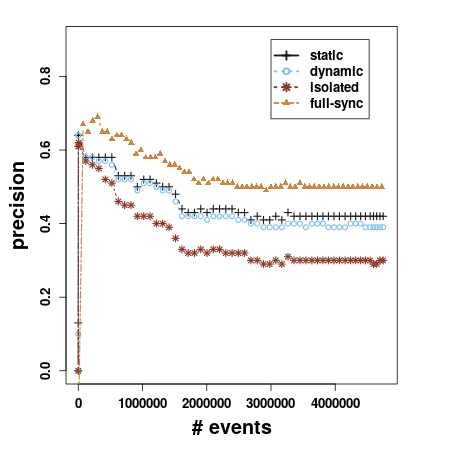
\includegraphics[width=\textwidth]{chapters/figures/precision_p1.png}
	
	\caption{Precision scores with respect to the number of input events over time for $\mathcal{P}_1$.}
	\label{fig:precsions}
\end{figure}

\subsection*{Experimental results} Figure ~\ref{fig:precsions} depicts the average precision scores of predictions models (one prediction model per vessel) of all synchronization modes for the first pattern $\mathcal{P}_1=Sailing$, namely, isolated without synchronization, continuous (full-sync), static, and our recommended approach based on the dynamic synchronization scheme. It can be clearly seen that all methods of distributed learning outperform the isolated prediction models. The hypothetical method of full continuous synchronization has the highest precision rates, while the static and dynamic synchronization schemes have close precision scores. Consequently, dynamic synchronization is not much weaker than the static synchronization, but requires much less communication, as explained below.
 

 
\par Figure ~\ref{fig:comm} provides the amount of the accumulated communication that is required by the three modes of the distributed online learning, while the isolated approach does not require any communication between the predictors. These results are shown  for $\mathcal{P}_1$.  As expected, a larger amount of communication is required for the continuous synchronization comparing to the static and dynamic approaches. Also, it can be seen that we can reduce the communication overhead by applying the dynamic synchronization protocol (a reduction by a factor of 100) comparing to the static synchronization scheme, even with a small variance threshold $\Delta=2$. Furthermore,  the dynamic  protocol is still preserving a close predictive performance to the static one (see Figure ~\ref{fig:precsions}).  Therefore, we will only consider the dynamic synchronization and the isolated approach in the  evaluation of the second pattern.

\begin{center}
	
	\begin{figure}[]
		
		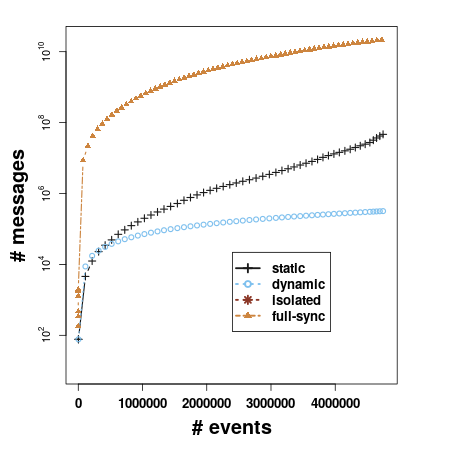
\includegraphics[width=\textwidth]{chapters/figures/messages_p1.png}
		
		\caption{Commutative communication with respect to the number of input events over time for $\mathcal{P}_1$.}
		\label{fig:comm}
	\end{figure}
\end{center}




\begin{center}
	
	\begin{figure}[]
		
		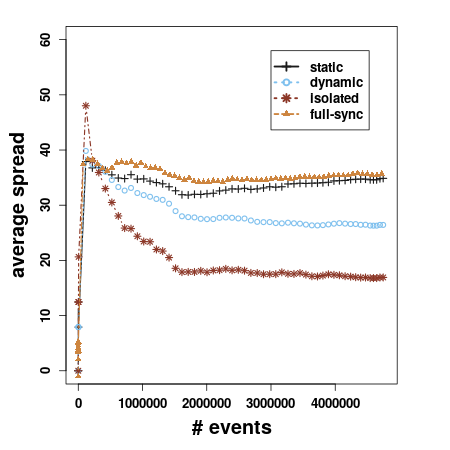
\includegraphics[width=\textwidth]{chapters/figures/spread_p1.png}
		
		\caption{Average spread value for $\mathcal{P}_1$.}
		\label{fig:spread}
	\end{figure}
\end{center}

 \begin{figure}[]
	
	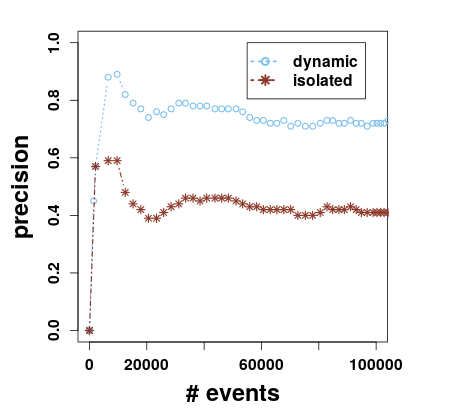
\includegraphics[width=\textwidth]{chapters/figures/precision_p2.png}
	
	\caption{Precision scores of $\mathcal{P}_2$  for \textit{PLEASURE CRAFT} vessels.}
	\label{fig:precsions_p2}
\end{figure}

\par In Figure ~\ref{fig:precsions}, we also noted that the precision is going down in a first phase and stabilizes then.  This seems to be counter-intuitive, as the models should improve when getting more data up to a certain point. For explanation, we have investigated the effect of the distributed synchronization of the prediction models on the average spread value, Figure  ~\ref{fig:spread}  shows the spread results for all approaches. It can be seen that the spread is higher for the distributed learning based methods comparing to the isolated approach. Furthermore, the average spread is decreasing over time until convergence, as result of confidence increase in the models. This may explain the drop in the precision scores from the beginning until reaching the convergence. We will investigate further in the interrelation between precision and spread in future work. 


\par For the second, more complex pattern ($\mathcal{P}_2$), we have found that the precision was worse for a distributed model generated over all vessels than in the model created for each vessel in isolation. This indicates that there is no  global model describing the behavior of all models consistently. However, when looking at specific groups of vessels, we achieved an improvement in terms of precision. As initial experiment, we only enable the synchronization of the prediction models associated with vessels that belong to the same vessel class. Currently, this change is technically performed by an extra filter step that passes only one type of vessels, while multiple runs of the system are required for all vessel types. For example, Figure ~\ref{fig:precsions_p2} shows the precision scores for vessels of class \textit{PLEASURE CRAFT}. An interesting observation is that the dynamic synchronization approach still has  a higher precision scores than the isolated approach. We will further investigate the effect of groupings and more patterns in future work.







%\par In Table ~\ref{tab:recall}, we present the mean of the recall scores for the both patterns in the all approaches It can be seen that the different approaches have a close recall scores, while the most frequent pattern ($\mathcal{P}_1$) has a lower recall than $\mathcal{P}_2$.
%
%\begin{table}[h]
%	\caption{Average recall for  $\mathcal{P}_1$ and $\mathcal{P}_2$.}
%	\label{tab:recall}
%	\begin{tabular}{lcc}
%		\toprule
%		Approach &Mean recall for $\mathcal{P}_1$ &Mean recall for $\mathcal{P}_2$\\
%		\midrule
%		isolated & 0.1707  &0.947 \\
%		static & 0.1754  &  0.960 \\
%		dynamic & 0.174  & 0.0.964 \\
%		full-sync & 0.1817  & 0.972 \\
%		\bottomrule
%	\end{tabular}
%\end{table}


 

	\chapter{Discussion}
\label{chapter:discussion}

	
\chapter{Conclusion and Future Work}
\label{chap:conclusions}

In this chapter, we discuss the results of our system, and some of the aspects of underlying method. Also we give some proposals for future work.




\section{Conclusion}
%In this paper, we have presented a system that provides  a distributed pattern prediction over multiple large-scale event streams of moving objects (vessels). The system uses the event forecasting with Pattern Markov Chain (PMC) \cite{alevizos2017event} as the base prediction model on each event stream, and it applies the protocol for distributed online prediction \cite{kamp2014communication} to exchange information between the prediction models over multiple input event streams.  Our proposed system has been implemented using Apache Flink and Apache Kafka, and empirically tested against large real-world event streams related to trajectories of moving vessels. As future work, we will investigate the effect of grouping the input event streams on the predictive performance of our proposed system. Furthermore,  we will study the interrelation between precision and spread scores.



\section{Future Work}
%\begin{itemize}[noitemsep]
%	\item In some practical applications the input event streams may belong to different distributions, we propose to divide the input event streams into similar groups, in order to combine the corresponding predictions models to construct a representative global model in each group. The aggregation operation refers to the synchronization operation (e.g., joint average of the local models) in the distributed online learning protocol, which is performed by a central coordinator that constructs and distributes a global prediction model for the input event streams based on the  local models.
%	\item temporal patterns 
%	\item another communication media  
%	\item theoretical analysis of dynamic protocol 
%	\item another transition probabilities learning technique 
%	\item another weighted sync operator
%	
%	
%	%	 it seems that predicted patterns currently concern individual objects (hence each one is monitored by a distinct predictor), although in reality there may be interactions and correlations among moving objects. As a future research direction, perhaps it would be worth briefly discussing whether and how this method could be extended to handle such correlated events involving multiple objects (e.g., a group of vessels heading to a place).
%	
%	
%\end{itemize}

	
	\FloatBarrier
	
	%\begin{singlespacing}
	%    \printbibliography
	%\end{singlespacing}
	\bibliographystyle{agsm}
	\bibliography{bmda-paper-bibliography,forecasting} 
\end{document}

